\newchapter{Block Merging for Re-Pair}{chap:remerge}

Phrase browsing techniques become more
important as document size increases.
When character-based \repair was introduced in 
\chapref{chap:repair}, the largest document processed by
\repair was a \mib{20} document, \wsja.  
Limitations on computer memory prevent significantly larger
documents being handled by \repair.
The space analysis for \repair (\secref{subsec:repair-space},
from \pgref{subsec:repair-space}) showed that 
its memory usage is linear to the length of the
message.  However, the analysis also showed that the constant 
factor is high.  For example, a \mib{100} message would 
require more than \gib{1} of memory for the sequence alone.

While the goal of \prepair was to align words in a document
for the purpose of browsing, both word-based and 
punctuation-aligned \repair also 
reduce the memory requirements of \repair.  \prepair separates
a message into multiple streams, including a word sequence
stream.  In the previous chapter,
it was shown that the parsing of \wsja by \prepair yielded
roughly one word token for every 5 characters in
the message for \repair.
The \wsja document of 20 million symbols
(characters) is transformed into a word sequence of just over
3 million symbols (references to the word lexicon).  Moreover,
the shorter input into \repair has a beneficial effect on the
overall compression time, even through the set of primitives 
increases in size.  
When character-based \repair is applied to \wsja, 
88.5 seconds is required (\tabref{tab:repair-time}, 
\pgref{tab:repair-time}).  However, word-based
\repair requires only 19.6 seconds 
(\tabref{tab:prepair-wordtime}, \pgref{tab:prepair-wordtime}).
(These times exclude the costs in parsing and entropy 
coding of the sequences and modifiers, which together
add 1.6 and 16.4 seconds back on to the execution
costs of character-based and word-based
\repair, respectively.)

In this chapter, the problem of using \repair on longer 
messages is considered.  The solution proposed
involves an initial partitioning of the
message into blocks, followed by the processing of each 
block by \repair.  The division of a message into
$b$ blocks presents problems for
browsing and compression.  
The challenge is to provide
post-processing steps for \repair 
that merge multi-block outputs, thereby solving these problems.

The remainder of this chapter is structured as follows.  The
creation of blocks using \repair is discussed in 
\secref{sec:remerge-blocks}.  The subsequent merging of blocks occurs
in three phases.  The first phase, described in 
\secref{sec:remerge-1}, merges the $b$ phrase hierarchies into
a single one.  \secref{sec:remerge-2}
describes phase 2, which employs the newly formed
phrase hierarchy to identify pairs of symbols for 
further replacement.  Then, \secref{sec:remerge-3} outlines the
third phase, which re-examines the sequence
to identify pairs of symbols that have not yet been represented
by any symbol in the phrase hierarchy.  In order to simplify the
discussion in this chapter, character-based \repair
is used for demonstrating the three phases.
\secref{sec:remerge-palign} explores the
changes required to each of these three phases in order
to accommodate punctuation-aligned \repair.  
\secref{sec:remerge-expt} provides 
experiments that demonstrate the efficiency and effectiveness
of block merging.  \secref{sec:remerge-append} describes how
text can be appended to a compressed document by extending
the block merging technique.  \secref{sec:remerge-summary} 
concludes the
chapter by discussing the trade-offs that exist with block
merging.

\newsection{Creating Blocks}{sec:remerge-blocks}

To sidestep memory limitations, many compression systems partition
large messages into blocks, and then process each block
independent of neighbouring blocks.  The \gzip compression
system implements an input buffer whose size is fixed for all
documents, limiting the maximum block size.
On the other hand, \ppmd and 
\bzip create blocks according to options
supplied by the user.  The \ppmd implementation used as a reference
point in this thesis ends the current block
when the maximum amount of memory specified by the user has
been exhausted, and compression is simply restarted from a 
``know nothing'' state.  The \bzip system allows 
the user to specify one of a set of block sizes.

The \bzip approach is also adopted by \repair for
large messages.  An explicit input block
size is supplied by the user, which specifies that the
message be divided into $b$ blocks, with all blocks
equal in size, except for the last one.
Each block is then compressed
independently using \repair, to produce $b$ phrase hierarchies and $b$ 
reduced sequences.

The forceful separation of a message into blocks for 
compression presents three problems for browsing and 
compression.  First, browsing 
multiple phrase hierarchies simultaneously is difficult,
and as cumbersome as physically browsing multiple books 
at the same time.
Second, since \repair selects phrases from each block
without any information gained through the compression of
previous blocks, it is likely that partitioning a uniform
file produces shorter phrases.  The maximum
generation of symbols in the phrase hierarchies would
be less than if the file is compressed as one block.
Lastly, not only does the quality of phrases worsen, but
compression degrades.
As the block size decreases, more blocks are produced.  Across
any two blocks, information is duplicated
in the phrase hierarchies and in the preludes
in the final entropy coded sequence.

The effect blocks have on phrase quality and compression 
is verified by experiments using the \wsjb file
described in \chapref{chap:tc}.  Recall that the file
is \mib{508} in size and that the \wsja from 
earlier experiments was derived from the first \mib{20}.
In the experiments, \wsjb was compressed using 
character-based \repair and block sizes ranging from 
\mib{1} to \mib{32}.  Coding of the sequence was handled
by the Huffman coder, \shuff, with each block entropy coded
independently of others.
The results from these experiments are shown in 
\tabref{tab:remerge-charblocks} and 
\figref{fig:remerge-charblocks}.

\tab{ccccc}
{\multirow{2}*{Block size} & Length of      & Maximum    & Number of symbols & \repair time \\
                           & longest phrase & generation & in phrase hierarchies  & (s) \\}
{
\D\mib{1}    &           3,094 &         25 &        16,189,378 &  1,969.9 \\
\D\mib{2}    &           3,094 &         27 &        13,474,410 &  2,033.7 \\
\D\mib{4}    &           3,094 &         29 &        11,367,932 &  2,092.2 \\
\D\mib{8}    &           4,970 &         28 &       \D9,668,774 &  2,171.1 \\
\mib{16}   &           4,970 &         29 &       \D8,306,278 &  2,275.6 \\
\mib{20}   &           4,970 &         31 &       \D7,948,461 &  2,323.3 \\
\mib{32}   &           4,970 &         31 &       \D7,215,594 &  2,448.0 \\}
{Statistics from applying character-based \repair on \wsjb
by partitioning with block sizes ranging from \mib{1} to \mib{32}.
The second and third columns list the length of the longest
symbol (in number of primitives) and the maximum generation
of all of the blocks, respectively.  The fourth column tabulates the total
number of primitives and phrases across all blocks.  The last
column shows the execution times of \repair, excluding the
entropy coding of the sequence.}
{Statistics from block-wise character-based \repair (\wsjb)}
{tab:remerge-charblocks}

\fig{\includegraphics*{./wsj-char-repair.eps}}
{Compression ratios from applying character-based \repair
on \wsjb by partitioning with various block sizes.  Also shown are
results from applying the \gzip, \bzip, and \ppmd compression
systems.}
{Compression ratios from block-wise character-based \repair (\wsjb)}
{fig:remerge-charblocks}

\tabref{tab:remerge-charblocks} shows that as the block
size increases, the overall quality of the phrase 
hierarchy improves since \repair is able to find longer phrases.
In the fourth column, the total number of symbols 
in all of the phrase hierarchies
decreases as the block size increases.  
Finally, in the last column, the
time for \repair to process the same file (excluding entropy
coding), averaged over three trials, increases
with the block size.  Since \shuff performs roughly the 
same amount of work irrespective of block size, the time taken
for coding remains the same.

\figref{fig:remerge-charblocks} depicts compression
effectiveness as a function of block size.  The division of
the output bits between the phrase hierarchy,
the compressed sequence prelude, and the 
compressed sequence codes are also shown.  Three horizontal
lines indicate the compression effectiveness of \gzip,
\bzip, and \ppmd on \wsjb, taken from \tabref{tab:tc-bpc} on
\pgref{tab:tc-bpc}.  Note that a comparison between
these three systems and \repair is unfair given that \repair 
is using more memory.  Of the four systems, \gzip performs
the worst, even with the {\texttt {-9}} option, since it 
creates a context window of only \kib{32}.  
With the {\texttt {-9}} option, \bzip creates blocks of \kib{900},
which is comparable to the smallest \mib{1} block size of \repair
shown in the graph.
The \ppmd system with \mib{255} of memory and a seventh
order model achieves the best compression overall.  
Clearly, compression effectiveness suffers 
when smaller block sizes are used by \repair, because 
symbols in the phrase 
hierarchy and codewords in the compressed sequence prelude
are duplicated.

In order to minimise the problems with phrase browsing and
compression effectiveness when \repair processes a message
in blocks, a block merging scheme called \remerge has been
designed as a post-processing step.  \remerge 
operates in phases, as shown in \figref{fig:remerge-phases}.  
These phases can be arranged into different configurations,
yielding five methods labelled method A to method E, as
shown.  The only required phase is phase 1, which is applied
immediately after \repair.  Then either of two alternative second
phases is used, phase 2a or phase 2b.  If phase 3 is
required, it is performed last.  The five combinations of these
phases represent the trade-offs that exist between execution
time of \remerge, compression effectiveness, and phrase
quality, as detailed in experiments later.

\fig{\input{./remerge-phases.pstex_t}}
{The three phases of \remerge and the combinations in 
which they are applied.  Two alternatives to the 
second phase of \remerge exists, labelled phase 2a and
phase 2b.  Five combinations of the \remerge phases 
are possible, labelled A to E, on the right.  The two outputs of
\repair are required by every \remerge phase, even though
they may not be modified by every phase.  So, a line
represents both streams.  Entropy coding of the 
reduced sequence is performed when \remerge has completed
every necessary phase.}
{Combinations of \remerge phases}{fig:remerge-phases}

Before discussing each phase, the notation introduced in 
\chapref{chap:repair} needs to be extended.  As before,
the number of primitives and phrases in a phrase hierarchy
are $|\Sigma|$ and $|\rho|$, respectively.  The phrase
hierarchy is denoted as $\Ph$, and the sequence as $\Seq$.
The total number of primitives and phrases in the phrase
hierarchy can be represented as $|\Sigma| + |\rho|$ or
$|\Ph|$.  The number of symbols in the
sequence is $|\Seq|$.  Let
$\Ph_1$ and $\Ph_2$ 
represent initial phrase hierarchies before any phase, and
$\Ph'$ represent the final
phrase hierarchy after the same phase.  Their corresponding 
sequences are $\Seq_1$, $\Seq_2$, and 
$\Seq'$.  When a symbol $\alpha$ 
is expanded, it becomes a string of primitives with a
length equal to $|\alpha|$.  In a string, 
a vertical bar (\textbar) is used to indicate
the division between the expanded left component and the
expanded right component (for example, ``wood{\textbar}chuck'').

The next three sections describe the three phases of \remerge
in detail.

\newsection{Merging Phrase Hierarchies}{sec:remerge-1}

The first phase of \remerge carries out a pair-wise 
merging of blocks via a series of passes.  Each pass 
halves the number of blocks, meaning that for an initial
message of $b$ blocks, $\lceil \log_2 b \rceil$
passes are required.  During each pass, the union of the
pair of phrase hierarchies, $\Ph_1$ 
and $\Ph_2$, is formed to produce $\Ph'$.  
After the two phrase hierarchies
are merged, the sequences $\Seq_1$ and 
$\Seq_2$ are modified to ensure that each symbol refers 
to $\Ph'$ and not their respective phrase 
hierarchies.  Afterwards, $\Seq_1$ and $\Seq_2$ are concatenated 
together.

Initially, phase 1 decodes both phrase hierarchies.  
They are then merged one generation at a time, with duplicate
phrases that have equal left and right components removed.  
Then, each symbol
is expanded into a string of primitives.  The phrase hierarchy
is sorted by these strings, producing a temporary phrase
hierarchy, $\Ph^*$.  With the strings sorted, duplicate symbols
that exist across and within generations, but with different 
components, can also be identified and removed.  Recall from 
\pgref{memo:repair:phdups} that when a message (or in this
case, a block) is processed by \repair, duplicates may occur
within the phrase hierarchy which have different components.  For
example, one symbol may expand to ``a{\textbar}aa'' while
another symbol may expand to ``aa{\textbar}a''.  The merging
of two phrase hierarchies occurs in two steps in order to
reduce the size of $\Ph^*$.  

The \repair decompressor, \despair, also expands phrases into
primitives.  However, since symbols are expanded into primitives
only as needed, \despair uses a buffer of recently 
decoded symbols as a trade-off between execution time and 
memory space (\tabref{tab:repair-despair}, 
\pgref{tab:repair-despair}).  The
needs of phase 1 of \remerge differs from that of \despair.
In order to sort the strings for $\Ph^*$, ideally, all strings
have to be available for sorting at once, and therefore all
need to be expanded beforehand.
But simply decoding every symbol could potentially occupy
memory proportional to the length of the original message.
Phase 1 of \remerge
(and subsequent phases which require the phrase hierarchy
to be expanded) take an alternative approach which expands
symbols starting from the last generation of symbols.  
Only symbols 
which are not used as a component of any other symbol are
expanded.  As a symbol is expanded, all
symbols which it is composed of, either directly or
indirectly, refer to the substrings of the expanded string 
instead.  This approach ensures that a minimum amount
of memory is taken up by the strings, while all of them are 
available for sorting and other operations in later \remerge
phases.

When two or more symbols in $\Ph^*$ have been found
which expand to identical strings, the one with the lower
generation is retained.  When a symbol has one of its components 
removed, it must reference the retained duplicate as
a component instead.  The symbol's generation
number also decreases accordingly.  As a result, a cascading effect
occurs, and symbols that refer to a removed symbol, either
directly or indirectly, shift to lower generations.  The overall 
result is the reduction of gaps in the phrase hierarchy.  After 
the removal of duplicates, the symbols in the phrase hierarchy
are sorted in generation and chiastic slide value order to form
$\Ph'$, for the interpolative coding stage.

\figref{fig:remerge-example1} shows an example of \remerge phase 
1. The following message is compressed with \repair using blocks
of 17 characters:  $\underline{\text{woowoodwoodywoody}}
\overline{\text{woodywood}}$.  
Two blocks are created by \repair, as shown with the underline and
overline.  Their respective lengths are 17 characters and 9 
characters.  When \repair is applied to these two blocks 
independently, two sets of phrase hierarchies and sequences are
produced, as shown in \subfigref{fig:remerge-example1}{a} and 
\subfigref{fig:remerge-example1}{b}.
In the example, the symbols in each of these phrase 
hierarchies are expanded immediately only for illustrative 
purposes.   
To the right of each expanded symbol 
is its generation.  The two phrase hierarchies are
merged so that duplicates with the same components are
removed.  At this stage, the algorithm expands each
symbol into primitives and sorts each string, producing
$\Ph^*$.  As \subfigref{fig:remerge-example1}{c} shows,
the duplicate ``wood'' exists and the higher generation of
the two is removed.  This affects the fourth generation phrase
``woody'' by shifting it into the third generation.  
\subfigref{fig:remerge-example1}{d} shows the final merged
phrase hierarchy, $\Ph'$, sorted in generation and 
chiastic value order.  Below the phrase hierarchy is 
$\Seq'$, created from the concatenation of the two
initial sequences and renumbered so that it refers to the
final phrase hierarchy.

\fig{
\begin{tabular}{cccc}

\multicolumn{1}{c}{$\Ph_1$} & \multicolumn{1}{c}{$\Ph_2$} & \multicolumn{1}{c}{$\Ph^*$} & \multicolumn{1}{c}{$\Ph^\prime$} \\

\begin{tabular}[t]{lc}
0 $\rightarrow$ d & 0 \\
1 $\rightarrow$ o & 0 \\
2 $\rightarrow$ w & 0 \\
3 $\rightarrow$ y & 0 \\
4 $\rightarrow$ o{\textbar}o & 1 \\
5 $\rightarrow$ w{\textbar}oo & 2 \\
6 $\rightarrow$ woo{\textbar}d & 3 \\
7 $\rightarrow$ wood{\textbar}y & 4 \\
\end{tabular}

&

\begin{tabular}[t]{lc}
0 $\rightarrow$ d & 0 \\
1 $\rightarrow$ o & 0 \\
2 $\rightarrow$ w & 0 \\
3 $\rightarrow$ y & 0 \\
4 $\rightarrow$ o{\textbar}d & 1 \\
5 $\rightarrow$ w{\textbar}o & 1 \\
6 $\rightarrow$ wo{\textbar}od & 2 \\
\end{tabular}

&

\begin{tabular}[t]{lc}
d & 0 \\
o & 0 \\
o{\textbar}d & 1 \\
o{\textbar}o & 1 \\
w & 0 \\
w{\textbar}o & 1 \\
w{\textbar}oo & 2 \\
wo{\textbar}od & 2 \\
\sout{woo{\textbar}d} & \sout{3} \\
wood{\textbar}y & 4 \\
y & 0 \\
\end{tabular}

&

\begin{tabular}[t]{lc}
0 $\rightarrow$ d & 0 \\
1 $\rightarrow$ o & 0 \\
2 $\rightarrow$ w & 0 \\
3 $\rightarrow$ y & 0 \\
4 $\rightarrow$ o{\textbar}d & 1 \\
5 $\rightarrow$ o{\textbar}o & 1 \\
6 $\rightarrow$ w{\textbar}o & 1 \\
7 $\rightarrow$ w{\textbar}oo & 2 \\
8 $\rightarrow$ wo{\textbar}od & 2 \\
9 $\rightarrow$ wood{\textbar}y & 3 \\
\end{tabular}

\\ \\

$\Seq_1 =$ [ 5 6 7 7 ] & $\Seq_2 =$ [ 6 3 6 ] & & $\Seq^\prime =$ [ 7 8 9 9 8 3 8 ] \\

\multicolumn{1}{c}{(a)} & \multicolumn{1}{c}{(b)} & \multicolumn{1}{c}{(c)} & \multicolumn{1}{c}{(d)} \\

\end{tabular}
}{The merging of two phrase hierarchies using \remerge phase
1.  Below the two initial phrase hierarchies and the final
phrase hierarchy are their respective sequences.  Vertical
bars (\textbar) indicate the division between the left and
right components of an expanded symbol.
Also shown is the intermediate phrase hierarchy, $\Ph^*$,
and the removed duplicate, ``woo{\textbar}d''.  Symbols
from every phrase hierarchy have been expanded into 
primitives, with each symbol's generation shown on the
right.}{\remerge phase 1 example}{fig:remerge-example1}

In order for $\Ph^*$ to be formed, symbols that are not 
referred to by a higher generation symbol are expanded.  This
is depicted by \figref{fig:remerge-expandstr} for
the example of \figref{fig:remerge-example1}.
In \figref{fig:remerge-expandstr}, the symbols
have been rearranged into a directed acyclic graph, with a
level in the graph corresponding to a particular generation.
The symbols with the highest generation are at the top of the
figure, while primitives are lined up along the bottom.
Directed edges are added from each phrase to its two 
components, except for the primitives which have no edges 
emanating from them.  

\fig{\includegraphics*{./expandstr.eps}}
{The phrase hierarchy of \subfigref{fig:remerge-example1}{c},
showing the two symbols that each symbol depends on.  
Symbols are arranged with the primitives along the bottom, 
and the highest generation phrase at the top.  Two phrases
are not used by any other symbol, ``wo{\textbar}od'' and
``wood{\textbar}y''.}
{Symbol dependencies for $\Ph^*$}
{fig:remerge-expandstr}

The symbol expansion by \remerge phase 1 starts from the 
highest generation symbol with the greatest chiastic slide
value in that generation.  The equivalent in the 
hierarchical graph representation is to commence
from the top of the graph, and then proceed toward the
primitives, a level at a time.  As \figref{fig:remerge-expandstr}
shows, the order within a level is unimportant, since 
no symbol can depend on other symbols within the 
same generation.  With the directed graph, expansion into 
primitives can be summarised as first searching 
level-by-level to find a symbol to expand, skipping those
that have already been expanded.  Once a node without
a directed edge leading to it has been identified, all of its 
descendents are ``decoded'' in a depth-first fashion by 
making each descendent refer to the higher generation node.
In the example, when the fourth generation symbol, ``wood{\textbar}y''
is first encountered, it is expanded.
Then, all symbols that refer to ``wood{\textbar}y'', 
either directly or indirectly, 
are ``expanded'' by making the lower generation symbols 
refer to parts of the expanded
string and by recording the length of the substring.  
Note that in this example, in order
to expand the entire phrase hierarchy, only two symbols, 
``wood{\textbar}y'' and ``wo{\textbar}od'' have to be 
explicitly expanded.
Finally, note that after $\Ph^*$ has been sorted and
duplicates removed, some symbols may be deleted
even though their expansion is needed by a lower generation
symbol.  Because of this, it is important that symbols in $\Ph^*$
are not actually removed during phase 1, but simply ignored 
when $\Ph'$ is built.

The amount of memory that this phase takes is proportional
to the size of the input and output phrase hierarchies.  Enough
space is required to keep $\Ph_1$, $\Ph_2$, and $\Ph^*$
in memory.  To minimise duplication in memory, the final phrase 
hierarchy can be drawn from $\Ph^*$.  
Additional space is also
required for the expansion of primitives, while the concatenation and
renumbering of the sequences can be performed without
keeping any symbols in memory.  The space requirements of phase 1
is an improvement to \repair because the memory usage
is proportional to the size of the phrase hierarchy, and not
the length of the initial sequence.

Excluding the costs of sorting, phase 1 operates through a 
series of linear passes over the phrase hierarchies.  First,
the phrase hierarchies are merged a generation at a time by
inserting symbols from $\Ph_1$ into a hash table and then 
comparing each symbol in $\Ph_2$ with the hash table entries.
When the two initial phrase hierarchies are merged, each symbol
is expanded by performing another pass over the $|\Ph^*|$ 
symbols.  Once the symbols are
sorted, a third linear pass over $\Ph^*$ is required to 
eliminate duplicates.  A final sort by generation number 
and chiastic slide value prepares the phrase
hierarchy for interpolative coding.  The initial sequences are 
renumbered and concatenated, with
buffering  required only for minimising disk accesses.
Combining two phrase hierarchies requires time proportional to
$|\Ph_1| + |\Ph_2| + 2|\Ph^*| + |\Seq'|$, not including the two
sorts that are performed.  This amount of time is required
for each of the $\lceil \log_2 b \rceil$ merges of a compressed
message of $b$ blocks.

The aim of phase 1 is to merge the phrase
hierarchies of every block into a single, unified phrase
hierarchy, while also removing any duplicate symbols.  
The relative sizes of the initial, intermediate,
and final phrase hierarchies can be summarised as follows:
$\text{max}(|\Ph_1|, |\Ph_2|) \leq |\Ph'| \leq |\Ph^*| \leq |\Ph_1| + |\Ph_2|$.
After $\lceil \log_2 b \rceil$ iterations of phase 1,
all of the phrase hierarchies have been merged and
all of the sequences have been concatenated.  Effectively, 
phase 1 has merged all of the blocks in the reduced message 
and the phrase hierarchy can be browsed.

While phase 1 makes phrase browsing feasible and
improves compression effectiveness, even better 
compression can be obtained.  For example, in the final sequence 
in \subfigref{fig:remerge-example1}{d}, the pair
of symbols [~8~3~] in $\Seq'$ can be replaced by a single symbol, [~9~].  
The next section describes phase 2 of \remerge, which 
shifts the attention from the phrase hierarchy to the 
sequence, to try to catch such redundancies.

\newsection{Identifying Old Symbol Pairs}{sec:remerge-2}

After the phrase hierarchies have been merged, pairs of 
symbols may appear in the concatenated 
sequence that are now candidates for replacement.  For example,
if $\alpha$$\beta$ exists twice in block 1, but once in
block 2, it would have been recognised as a phrase in the first block,
but not in the second.
The concatenated sequence needs to be checked to ensure
no pairs of symbols exist that are already represented by
symbols in the merged phrase hierarchy.

Identifying symbol pairs in the initial sequence that already 
have a
corresponding rule for replacement is the motivation for
phase 2.  Phase 2 reduces the length of the sequence, but makes
no changes to the phrase hierarchy.  As with \repair, the goal
of this phase is to minimise the length of the sequence.  Since
phase 2 is separated from the coder, no guarantees can be made
that reducing the length of the sequence also improves compression
effectiveness.
However, phase 2 improves the usefulness of the phrase browsing
interface.
Suppose a user is examining a symbol $\gamma$, which expands
to the pair $\alpha$$\beta$.  Phase 2 ensures that more  
occurrences of this pair of symbols can be located with the
phrase browsing system.  Since this phase does
not alter the merged phrase hierarchy $|\Ph'| = |\Ph_1|$.  But
as the
aim of phase 2 is to reduce the length of the initial sequence,
$|\Seq'| \leq |\Seq_1|$.

Two methods of performing
phase 2 are explored in this section.  The first method, phase
2a, is biased towards efficiency, while the second method, phase
2b, favours compression effectiveness.  

\newsubsection{Efficient Sequence Reduction}{subsec:remerge-2a}

Phase 2a of \remerge determines replacements by performing a
single pass through the initial sequence $\Seq_1$.  As each 
symbol is processed in the pass, it is considered in combination 
with the immediately preceding symbol, and a replacement made
if the pair exists in the phrase hierarchy.

The steps for phase 2a are shown in \algref{alg:remerge-2a}.
First, a hash table of symbols is constructed,
with all phrases in the phrase hierarchy hashed
according to their two components, and collisions
handled by chaining.  Then, each symbol in $\Seq_1$
is processed as follows.  When a symbol $\alpha_i$ from the sequence 
is read, it is combined with its immediately preceding symbol
$\alpha_{i-1}$.  The pair $\alpha_{i-1}$$\alpha_i$ is 
searched in the hash table.
If a matching phrase $\gamma$ is found, then a
replacement is made.  Then $\gamma$ is combined
with its preceding symbol, the one that preceded $\alpha_{i-1}$.  
This continues until a replacement is no longer possible.  
Then, the next symbol 
in $\Seq_1$ is read and the process repeats.  Phase 2a completes 
when the end of $\Seq_1$ has been reached.  

\algo{\begin{minipage}{\textwidth}
\DontPrintSemicolon

\SetFuncSty{textnormal}
\SetArgSty{textnormal}
\SetDataSty{textnormal}

\SetKwInOut{Input}{input}
\SetKwInOut{Output}{output}

\SetKwFunction{searchHashTable}{searchHashTable}

\SetKwData{newsym}{$\gamma$}
\SetKwData{sym}{$\alpha_i$}
\SetKwData{prevsym}{$\alpha_{i-1}$}
\SetKwData{rep}{\var{replacement}}

\SetKwData{pone}{$\Ph_1$}
\SetKwData{pprime}{$\Ph'$}
\SetKwData{sone}{$\Seq_1$}
\SetKwData{sprime}{$\Seq'$}

\SetKwData{false}{{\textsc {FALSE}}}
\SetKwData{true}{{\textsc {TRUE}}}

\Input{\pone and \sone}
\Output{\pprime and \sprime}

\BlankLine

\lnl{algline:remerge2a:1}
\ForEach{symbol in \pone}{
\lnl{algline:remerge2a:2}
  insert symbol into hash table using its components \;
}

\BlankLine

\lnl{algline:remerge2a:3}
\For{$i < |\Seq_1|$}{
\lnl{algline:remerge2a:4}
  \rep $\leftarrow$ \true \;
\lnl{algline:remerge2a:5}
  \While{\rep $=$ \true}{
\lnl{algline:remerge2a:6}
    \newsym $\leftarrow$ \searchHashTable{\prevsym, \sym} \;
\lnl{algline:remerge2a:7}
    \If{\newsym found}{
\lnl{algline:remerge2a:8}
      \prevsym $\leftarrow$ \newsym \;
\lnl{algline:remerge2a:9}
      $i \leftarrow i - 1$ \;
\lnl{algline:remerge2a:10}
      \rep = \true \;
    }
\lnl{algline:remerge2a:11}
    \Else{
\lnl{algline:remerge2a:12}
      \rep = \false \;
    }
  }
}

\lnl{algline:remerge2a:13}
\pprime $\leftarrow$ \pone ;
\sprime $\leftarrow$ \sone \;

\lnl{algline:remerge2a:14}
\Return (\pprime, \sprime) \;
\end{minipage}
}{Algorithm for \remerge phase 2a.}
{\remerge phase 2a}{alg:remerge-2a}

The memory requirements of phase 2a include the phrase hierarchy,
without symbols expanded, and a buffer for the initial sequence.  
Since the replacement $\gamma$ is at least one generation
higher than $\alpha$ and $\beta$, the maximum number of consecutive
replacements cannot be more than the maximum symbol generation in the
phrase hierarchy.  Therefore, a buffer whose size is
equal to at least the maximum symbol generation is sufficient.
As experiments later show, applying character-based \repair
on blocks from \mib{508} of text 
produces a phrase hierarchy whose highest
symbol generation is 31.

With respect to execution time, phase 2a performs two main operations.
First, all of the symbols in the phrase hierarchy are inserted into
the hash table.  Second, every symbol is combined with its preceding
symbol for searching in the hash table.  If we assume that
the size of the hash table is selected so that the length of
the chains are about 1, then
accessing it during creation or searching
requires constant time.  So, the first operation can be
performed in $O(|\Ph_1|)$ time.  The second task requires 
$|\Seq_1|$ hash table look-ups when no replacements are
made.  If the number of replacements made is taken into account, 
then note that the most substitutions an input symbol
can participate in cannot be more than the highest symbol 
generation.  That is, if the highest symbol generation is $g$,
then the second task runs in $O(g|\Seq_1|)$.  After phase 2a
completes, the number of searches into the hash table can be given
as $|\Seq_1| + (|\Seq_1| - |\Seq'|) \leq g|\Seq_1|$.
A single replacement during phase 2a reduces 
the length of $|\Seq_1|$ by one symbol and adds one search 
operation into the hash table.  
As the sequence usually has more symbols than the phrase
hierarchy, the execution time of phase 2a is $O(g|\Seq_1|)$.

This phase of \remerge is able to locate all pairs of symbols in
the sequence that can be replaced.  Phase 2a is fast and
memory efficient, as demonstrated in experiments later in this chapter.

\newsubsection{Effective Sequence Reduction}{subsec:remerge-2b}

While phase 2a locates all pairs of symbols in the sequence
produced by phase 1, the choices made may not be the best.
A replacement now may prevent an even better replacement later
that ends up reducing the overall length of the sequence.
As an alternative to phase 2a, phase 2b
optimally re-parses the sequence using the merged 
phrase hierarchy as a reference point.  Phase 2b should not
be used in conjunction with phase 2a, as doing so 
achieves no benefit.

Phase 2b is based on work by \citet{kr89:cj}
and \citet{klein97:cj}, and involves the re-parsing, or 
recompression, of the original
message using phrases from a dictionary.  Like the previous
investigations in recompression, phase 2b converts the 
problem of compression to that of determining the single
source shortest path in a directed acyclic graph (DAG).  Unlike
the earlier work, phase 2b is tailored specifically for \repair,
in that it exploits the structure in the 
phrase hierarchy and sequence.

Phase 2b constructs a graph $G$
with a set of vertices $V$ connected by a set of edges $E$  
denoted as $G (V,E)$.  Each vertex $v_i \in V$ represents the
$i$th primitive in the original message.  An additional vertex is 
added to $V$ as a {\emph {sink node}}.  For a 
message of $n$ primitives, $V$ has $n + 1$ vertices.

Edges are attached to the vertices based on the strings in
the phrase hierarchy.  
Vertices are examined in the order dictated by the original
message, with the sink node being last.
A directed edge $e_j \in E$ is drawn from $v_i$ to $v_{i + k}$, 
for $k > 0$, if a symbol exists in the phrase hierarchy which,
when expanded, coincides with the $k$ primitives starting from
$v_i$ up to, and including, $v_{i + k - 1}$.
Since every primitive in the
message exists in the phrase hierarchy, every vertex has at 
least one edge leading to the next vertex, and the graph is 
guaranteed to be connected.  The vertex representing the 
last primitive has an edge leading to the sink node $v_{n + 1}$.
Every edge has a weight of one.

After all possible edges are added to $E$, a new sequence
$\Seq'$ is created by finding the shortest path
from $v_1$ to the sink node $v_{n + 1}$, thereby minimising the total number
of edges traversed.  Because the edges have unit cost, 
the shortest path can be determined 
through breadth-first search 
\citep{clrs01:book}, and represents the optimal parsing 
of the message using the phrase hierarchy, if optimality is measured
by the number of edges spanned.

\figref{fig:remerge-example2b-graph} shows a graph for
the merged phrase hierarchy and the beginning of the decoded
message from \figref{fig:remerge-example1}.  That phrase hierarchy has
been reproduced in \tabref{tab:remerge-example1-phsorted}, sorted 
in alphabetical
order.  In \figref{fig:remerge-example2b-graph}, the optimal 
parsing for the first 7 primitives consists of the two 
symbols 7 and 8, obtained by traversing the dashed edges.  

\tab{cl}
{
Phrase hierarchy & Expanded \\
index            & phrase \\
}
{
0 & d  \\
1 & o  \\            
4 & od \\            
5 & oo \\            
2 & w  \\            
6 & wo  \\           
7 & woo   \\         
8 & wood  \\         
9 & woody \\         
3 & y     \\
}{The final phrase hierarchy of \figref{fig:remerge-example1}, 
sorted in alphabetical order.  The indexes in the first column
refer to the positions of the symbols in the unsorted phrase
hierarchy.}{Final phrase hierarchy of \figref{fig:remerge-example1}
in sorted order}{tab:remerge-example1-phsorted}

\fig{\input{./example2b-graph.pstex_t}}
{A graph representation of part of the message from the example
of \figref{fig:remerge-example1}.  The symbols in
the final phrase hierarchy of that figure allow edges to be 
added.  The shortest path through these 8 vertices is shown 
as dashed lines.}
{Representing part of a message as a graph}{fig:remerge-example2b-graph}

If the phrase hierarchy is sorted, edges can be selected for $E$
through binary search.  For example, suppose
the vertex $v_1$ in \figref{fig:remerge-example2b-graph} is currently
being processed.  Let the string starting from this vertex, 
``woowoodw...'', be denoted as $\tau_1$.  
A binary search for $\tau_1$ in the phrase 
hierarchy would return ``woo'' as the longest match.  
By reducing
the number of significant primitives in $\tau_1$, other edges
from $v_1$ can be found, until the shortest edge of length 1 has
been located.  This process must be repeated for every vertex
in the graph.  

The cost of finding just the longest match for every vertex 
in a graph derived from a message of $n$ primitives
is $O (n \log_2 |\Ph_1|)$ string comparisons.
A slight improvement is possible when an index into the phrase
hierarchy is set up for the $|\Sigma|$
primitives to constrain the binary search.  
For example, the longest match for ``woowoodw...''
must exist between ``w'' and ``x'', assuming both exist as
primitives in the phrase hierarchy.  In the worse case, if 
every symbol begins with the same primitive, then such a data
structure would neither improve nor significantly
worsen the execution time.  While not implemented for the
experiments later, the size of the index could increase by
indexing on more than one primitive.

Phase 2b applies binary search with this index structure for primitives,
while also
exploiting other characteristics of the phrase hierarchy, and of
the symbols in the initial sequence.
There are four main steps to \remerge phase 2b, which are described
in the next few paragraphs.  The first step adds 
links to each symbol in the phrase hierarchy.  
The second step expands the initial sequence into 
primitives to form $V$.  Then, edges are added to $E$ in the
third step.  Finally, $\Seq'$ is output by 
determining the shortest path through the vertices.

\newsubsubsection{Additional links for the phrase hierarchy}{subsec:remerge-2b-step1}

Phase 2b assumes that each symbol in the phrase hierarchy
has been expanded into primitive strings and then
sorted on these strings.  
Three types of links are added to each symbol in the phrase 
hierarchy in preparation for phase 2b.  The three link types
for each symbol lead to a {\emph {primary prefix symbol}}, 
a {\emph {secondary prefix symbol}}, and a list of 
{\emph {extended symbols}}.

A symbol $\beta$ is a prefix of 
another symbol $\alpha$, if $|\beta| \leq |\alpha|$ and
the expanded string of $\beta$ coincides with the first 
$|\beta|$ primitives of $\alpha$.  A symbol $\beta$ 
is the {\emph {primary prefix symbol}} of $\alpha$ if $\beta$ is
the longest prefix symbol in the phrase hierarchy for $\alpha$.
A symbol $\beta$ is the {\emph {secondary prefix symbol}} 
of $\alpha$ if $\beta$
is the longest prefix of $\alpha$, starting from $\alpha$'s second 
primitive.  The primary and secondary prefix symbols of a primitive
are the empty symbol, $\lambda$.  
For example, in the phrase hierarchy of
\tabref{tab:remerge-example1-phsorted}, the symbol
``wood'' has ``woo'' and ``oo'' as its primary and secondary prefix
symbols, respectively.
As no two symbols in the phrase hierarchy expand to the 
same string after phase 1, 
every symbol is guaranteed to have exactly one symbol that 
serves either role.

The symbol $\beta$ is an {\emph {extended symbol}} of $\alpha$, if 
two conditions hold.  First, $\alpha$ must be the primary 
prefix symbol of $\beta$.  Second, for some primitive 
$\delta$, no symbol which is lexically smaller than $\beta$
exists which has the string $\alpha$$\delta$
as a prefix, where the juxtaposition of symbols represents string
concatenation.  According to this definition, the string $\alpha$$\delta$
does not have to exist in the phrase hierarchy, but this is possible
if $\beta$ is longer than $\alpha$ by one primitive.  For example, 
in \tabref{tab:remerge-example1-phsorted}, ``wood'' is an extended
symbol of ``woo'', where $\delta = \textrm{``d''}$.  

A symbol has a list of zero to at most $|\Sigma|$ extended 
symbols.  An extended symbol is 
recorded as a pair, of the form 
$(\delta, \beta)$, and ordered in the list according to
$\delta$.  The pair $(\delta, \beta)$ states that, for the 
current symbol $\alpha$, the primitive $\delta$ can be
appended to it, and the lexically smallest symbol 
in the sorted phrase hierarchy with this  
string as a prefix is $\beta$.  When the
list of extended symbols is non-empty, then a special 
pair of the form $(\epsilon, \beta)$ is added to the end.  This
pair, called an $\epsilon$-pair, indicates that in the 
lexically sorted phrase hierarchy,
no symbol has $\alpha$ as a primary prefix symbol at or 
after $\beta$.  Also, the symbol immediately before 
$\beta$ must have $\alpha$ as a primary prefix symbol.

\tabref{tab:remerge-example2b-longph} further clarifies the 
definition of extended symbols by demonstrating how they are
used.  The table shows a section of a sorted phrase hierarchy
from the symbol ``wo'' to ``work'', with the symbols expanded into
strings.  Also shown are every symbol's primary prefix symbol and
list of extended symbols.
Suppose $\tau_1 =$ ``woodcutters'' and, through methods described
below, the current prefix for $\tau_1$ is the string ``wood'', but
whether a longer one exists is unknown.
Since the first four primitives of ``wood'' match with $\tau_1$
and the next primitive in $\tau_1$ is available,
the longest match must exist between ``woodc'' and the lexically
largest symbol that has ``wood'' as a prefix symbol and is followed by a ``c''.  
These two boundaries can be established through two 
consecutive extended symbol pairs for the symbol ``wood''.
While a binary search within the search space allows a longer prefix
to be found for $\tau_1$, locating the longest prefix requires
this process to be repeated.  Rather than applying
binary search on the entire phrase hierarchy, extended symbols permit
sections of the phrase hierarchy to be isolated based on the 
primitives that have already been compared.

\tab{clcl}
{
Phrase & \multicolumn{1}{c}{Expanded} & Primary & \multicolumn{1}{c}{Set of extended} \\
hierarchy & \multicolumn{1}{c}{phrase} & prefix & \multicolumn{1}{c}{symbols} \\
index & & symbol & \\
}
{
...  &                &           & \\
999  & wo             & 847       & [ (``o'', 1000), (``r'', 1009), ($\epsilon$, 1121) ]\\
1000 & wood           & 999       & [ (``b'', 1001), (``c'', 1002), ($\epsilon$, 1008) ]\\
1001 & woodblock      & 1000      & \\
{\greybox {1002}} & woodcarving    & 1000      & \\
1003 & woodchip       & 1000      & \\
1004 & woodchuck      & 1000      & [ (``s'', 1005), ($\epsilon$, 1006) ] \\
1005 & woodchucks     & 1004      & \\
1006 & woodcraft      & 1000      & \\
{\greybox {1007}} & woodcut        & 1000      & [ (``t'', 1008), ($\epsilon$, 1009) ] \\
1008 & woodcutter     & 1007      & \\
1009 & work           & 999       & \\
...  &                &           & \\

}
{Binary search on the phrase hierarchy using
extended symbols.  The numbering for the index (first column) is
referred to by the third and fourth columns.  In the second column,
every symbol has been expanded into primitives, and the entire phrase
hierarchy has been sorted on this column.}{Binary searching a phrase
hierarchy using extended symbols}{tab:remerge-example2b-longph}

The steps performed for the example of 
\tabref{tab:remerge-example2b-longph} is as follows.  
The extended symbols of ``wood'' indicate that a ``c'' can be
appended to it.  The first such symbol is symbol 1002, 
``woodcarving''.  The last symbol that has ``wood'' as a primary
prefix symbol and ``c'' as the fifth primitive is 
``woodcut'', which is one symbol before the
$\epsilon$-pair to ``woodcutter''.  A binary search between
these two symbols, shown shaded in \tabref{tab:remerge-example2b-longph},
is performed next. 
Within this interval, all of these strings
have the same first five primitives.  However, not all of
them share the same primary prefix symbol.
The longest match within this search interval is
``woodcut'', but it is still not the longest match for $\tau_1$.
An attempt to extend ``woodcut'' using the next primitive, ``t''
is made.  It succeeds and a search interval of one symbol (1008)
is found.  This symbol cannot be
extended further, so the longest match for $\tau_1 =$ ``woodcutters'' is 
``woodcutter''.

As an example of primary prefix symbols, secondary prefix symbols,
and sets of extended symbols, \tabref{tab:remerge-phraselinks}
shows these links for the phrase hierarchy of
\tabref{tab:remerge-example1-phsorted}.  The first two columns of
the figure show the phrase hierarchy indexes and expanded strings.  
The next two columns show the primary and secondary
prefix symbols.  In the last column, the lists of
extended symbols are shown for symbols that are primary
prefix symbols of another symbol.
In case an $\epsilon$-pair points outside
of the phrase hierarchy, an extra symbol has been added at
position 10 of the phrase hierarchy.

\tab{clccl}
{
Phrase hierarchy & Expanded & Primary & Secondary & \multicolumn{1}{c}{Set of extended} \\
index & \multicolumn{1}{c}{phrase} & prefix & prefix & \multicolumn{1}{c}{symbols} \\
& & symbol & symbol & \\
}
{0 & d              & $\lambda$ & $\lambda$ & \\
1 & o              & $\lambda$ & $\lambda$ & [ (``d'', 4), (``o'', 5), y($\epsilon$, 2) ] \\
4 & od             & 1         & 0         & \\
5 & oo             & 1         & 1         & \\
2 & w              & $\lambda$ & $\lambda$ & [ (``o'', 6), ($\epsilon$, 7) ] \\
6 & wo             & 2         & 1         & [ (``o'', 7), ($\epsilon$, 8) ] \\
7 & woo            & 6         & 5         & [ (``d'', 8), ($\epsilon$, 9) ] \\
8 & wood           & 7         & 5         & [ (``y'', 9), ($\epsilon$, 3) ] \\
9 & woody          & 8         & 5         & \\
3 & y              & $\lambda$ & $\lambda$ & \\
10 & \multicolumn{4}{c}{(End of phrase hierarchy)} \\
}
{The additional symbol links required for the phrase hierarchy
before starting phase 2b.  Primary and secondary prefix symbols
are shown in the third and fourth columns, after the expanded 
symbols.  These symbols do not exist for primitives, and are 
indicated by the empty symbol, $\lambda$.
In the last column, sets of extended symbols are either
empty, or made up of at least two pairs, with the last pair
being of the form $(\epsilon, \alpha)$.  Note that the pair 
$(\epsilon, 7)$ of symbol 2 points to symbol 7 and not 10.
While symbols 7 to 9 start with ``w'', none of them have a 
primary prefix symbol of 2.}{Additional phrase hierarchy
symbol links}{tab:remerge-phraselinks}

Phase 2b requires the phrase hierarchy to be sorted by
strings of expanded symbols.  Then, symbols are linked
through a series of passes.  Primary prefix symbols are assigned
first by comparing each symbol with its immediately preceding
symbols.  When searching, the first prefix symbol located 
serves as the primary prefix symbol, due to the sorted order.  While
it is possible for a symbol to be compared with every symbol
before it, in practice, a match is usually found after a few 
strings have been checked.  
A second pass is done to attach
symbols to the lists of extended symbols, using the
primary prefix symbol links.  Each symbol adds or updates an
extended symbol pair to the list associated with its
primary prefix symbol.  A third pass makes use of the other two
types of links to assign the secondary prefix symbols.
With the phrase hierarchy
sorted according to expanded symbols, consecutive symbols are
expected to have the same, or similar, secondary prefix symbols.
This observation assists in the creation of this third link,
in the absence of re-sorting the phrase hierarchy from each
string's second primitive.

The three types of links add $6|\Ph_1|$
words of memory to the phrase hierarchy of phase~1.  
Every symbol in the phrase hierarchy has exactly one primary
prefix symbol and one secondary prefix symbol, each stored in
one word of memory.  An extended symbol pair requires two
words of memory, and there cannot be more than 
$|\Ph_1|$ of them.  As proof of this claim, note
that one of the conditions for $\alpha$ to be an extended
symbol of $\beta$ is that $\beta$ is the primary prefix of 
$\alpha$.  Since $\alpha$ has an unique primary prefix symbol,
each symbol in the phrase hierarchy participates as 
an extended symbol only once.
Finally, for each non-empty set
of extended symbols, there must be an extra $\epsilon$-pair
to end the list of pairs.
Each of these require two words of memory.  

\newsubsubsection{Decoding the sequence}{subsec:remerge-2b-step2}

After the symbol links have been established for the phrase 
hierarchy, the next step is to expand the symbols in $\Seq_1$ 
into $\tau$.  For a message of $n$ primitives, this operation
requires memory proportional to $n$.  Alternatively,
$\Seq_1$ can be decoded a symbol at a time so that the length of
$\tau$ is at least equal to the length of
the longest symbol in the phrase hierarchy, $\alpha_L$.

While expanding the sequence into $\tau$, the original symbols 
in $\Seq_1$ are maintained to improve search times later.  
Each vertex is augmented
with an {\emph {initial search position}}.  The initial
search position at vertex $v_i$ 
is a symbol which is guaranteed to be the lower bound in a binary search 
for the longest prefix for $\tau_i$.  For example, if $\tau_1$ is
the string ``woowoodw...'', then ``w'' is one possibility 
for $v_1$.  However, a longer initial search
position is possible if $\Seq_1$ is taken into account.  
When a symbol is decoded into primitives for $\tau_i$, 
the symbol may not represent the longest
match, but it may still be a better match than a single
primitive.  This is illustrated in 
\figref{fig:remerge-example2b-seq} using the final phrase 
hierarchy and sequence from \figref{fig:remerge-example1}.  The first two
symbols of $\Seq_1$ are
7 and 8.  The primitives at the beginning of the expanded
symbols acquire these 2 symbols as initial search
positions, as shown in the figure.

\fig{\input{./example2b-seq.pstex_t}}
{Example decoding of $\Seq_1$ into vertices, represented
as an array.  Each vertex keeps track of the primitive and an
initial starting position.}{Decoding $\Seq_1$
into vertices}{fig:remerge-example2b-seq}

The remaining initial search positions are initialised with
symbols representing single primitives.  However, each are
later replaced by the secondary prefix symbol of the 
preceding vertex, if it is longer.
For example, in \figref{fig:remerge-example2b-seq}, after
the longest edge representing ``woo'' is added to $v_1$,
its secondary prefix symbol is ``oo''.  This symbol replaces
the initial search position at $v_2$, which is the primitive
``o'' (shown shaded).

\figref{fig:remerge-example2b-seq} also demonstrates how
only the minimum number of
symbols need to be decoded for $\tau_i$.  If the
current vertex being processed is $v_1$, then since $|\alpha_L| = 5$
for \tabref{tab:remerge-phraselinks}, only two symbols need to
be decoded to create $\tau_1$ with a length of 7 primitives.
Additional symbols are decoded as phase 2b progresses through
$\tau$.

\newsubsubsection{Adding edges to the graph}{subsec:remerge-2b-step3}

After enough of the sequence has been 
decoded so that $|\tau_i| \ge |\alpha_L|$, edges are added to 
$v_i$, starting with the longest one.
The longest edge from $v_i$ is also the primary prefix of 
$\tau_i$.

Let the symbol $\beta$ represent the best prefix symbol so far and
$\delta$ be the primitive at position $|\beta| + 1$ in $\tau_i$.  
The symbol $\beta$ is initialised with the initial search position
of $v_i$, and is concatenated with $\delta$ for
searching in the extended symbols of $\beta$.  If the search is unsuccessful,
then $\beta$ is the longest match.  But if the search is successful,
two consecutive symbol pairs are retrieved, where the first one is
the pair $(\delta, \alpha)$.  These two pairs, $\alpha_\textrm{left}$
and $\alpha_\textrm{right}$, form an area within the
phrase hierarchy for binary search.  If the binary search fails,
the current version of $\beta$ is the longest primary
prefix.  If the search succeeds, then a longer string is returned.
The process repeats with this longer string by first 
extending it with its next primitive in $\tau_i$.

Once the longest edge has been determined and added, 
all shorter edges are located by repeatedly following prefix symbol 
links until the empty symbol ($\lambda$) is reached.  

\newsubsubsection{Determining the shortest path}{subsec:remerge-2b-step4}

The last step of phase 2b requires the calculation of the
shortest path through the graph.  Earlier, the number of symbols
in the sequence that have to be decoded was reduced by
noticing that only the first $|\alpha_L|$ primitives in $\tau_i$
are significant.  Another observation divides the expanded
sequence into segments in order to prevent the entire
message from being kept in memory.

A {\emph {segment}} is defined as being a sequence of 
vertices which begins and ends with {\emph {cut vertices}} 
(also called {\emph {choke points}}).
A cut vertex is a vertex which has edges starting or ending
at it, but no edges that bypass it.  The first vertex $v_1$
and the sink node $v_{n + 1}$ are both examples of cut 
vertices.  Other cut vertices also exist in most sequences
and can be taken advantage of.

Since no edges bypass a cut vertex, the shortest path
through the set of vertices must go through that vertex.  
Therefore, if the graph $G$ is processed in segments, no
loss in the optimal parsing of the message occurs.
The shortest path can be determined a
segment at a time, rather needing to have all of $V$ in
memory.

\figref{fig:remerge-example2b-cutvertex} demonstrates
how the first few primitives of 
\figref{fig:remerge-example2b-seq} are handled using
the phrase hierarchy and symbol links of 
\tabref{tab:remerge-phraselinks}.  Three pointers to the 
vertices are maintained:  \var{min}, \var{max}, and $i$.  The
vertex at position $i$ is currently being examined.  The \var{min}
pointer represents the beginning of the current segment,
while \var{max} points to the vertex that is reached by the
longest edge.
Whenever the vertex currently being examined 
meets \var{max}, a cut vertex has been found, as in
\subfigref{fig:remerge-example2b-cutvertex}{d}.

An examination of \figref{fig:remerge-example2b-cutvertex} reveals
an alternative method of performing phase 2b, which has not
been attempted.  Currently, at each step, the 
vertex at position $i$ is examined to determine all of the
edges that start from $i$.  Another way of performing phase 2b
is to determine all edges that end at $i$, instead.  This
method of conducting phase 2b has the potential of being more
memory efficient.  As edges are added, others may be removed
if a better way of reaching the current vertex $i$ has been
found.  At least one change to the current phase 2b algorithm is required
in order to use this proposed version.  While phase 2b requires the
phrases in the hierarchy to be
sorted in the forward direction, this proposed
version would require all of the strings to be reversed, and
then sorted.

\fig{
\begin{tabular}{c}
\input{./example2b-cutvertex1.pstex_t} \\
(a) \\
\input{./example2b-cutvertex2.pstex_t} \\
(b) \\
\input{./example2b-cutvertex3.pstex_t} \\
(c) \\
\input{./example2b-cutvertex4.pstex_t} \\
(d) \\
\end{tabular}
}
{Examining vertices to locate the next cut vertex.
The pointer $i$ indicates the vertex
that is being considered.  When $i$ coincides with the pointer
\var{max}, a cut vertex has been found, and the next segment is from
\var{min} to \var{max}.  Note that when $|\tau_i|$ is less than the
length of the longest symbol, more symbols need to be decoded,
as in the lower two figures.}{Adding edges and locating 
a cut vertex}
{fig:remerge-example2b-cutvertex}

The segment from \var{min} to \var{max} is processed by finding the
shortest path through the segment.
The shortest path through a segment is determined by using 
breadth-first search, 
which has a running time of $O(|V| + |E|)$ \citep{clrs01:book}.
After the shortest path
has been found, the symbols that represent that path are
added to the final sequence $\Seq'$.  At this
point, the memory taken up by the segment is released
before starting on the next segment with $i$ and \var{min}
starting from \var{max}.

\newsubsubsection{Analysing Phase 2b}{subsec:remerge-2b-alg}

The algorithm for phase 2b is shown 
in \algref{alg:remerge-2b}.  This algorithm excludes the sorting 
of the phrase
hierarchy by expanding symbols and the addition of symbol links
\algref{alg:remerge-2b} requires $\Ph_1$, $\Seq_1$, and the sorted
phrase hierarchy $\Ph_s$ as input.  At the end, $\Ph'$ and $\Seq'$
are produced by the algorithm.

\algo{\begin{minipage}{\textwidth}
\DontPrintSemicolon

\SetFuncSty{textnormal}
\SetArgSty{textnormal}
\SetDataSty{textnormal}

\SetKwInOut{Input}{input}
\SetKwInOut{Output}{output}

\SetKwFunction{binarySearch}{binarySearch}
\SetKwFunction{findExtendSymbol}{findExtendSymbol}
\SetKwFunction{addEdge}{addEdge}
\SetKwFunction{findShortestPath}{findShortestPath}

\SetKwData{leftside}{$\alpha_{\text{left}}$}
\SetKwData{rightside}{$\alpha_{\text{right}}$}
\SetKwData{minvar}{\var{min}}
\SetKwData{maxvar}{\var{max}}
\SetKwData{algdepth}{\var{depth}}
\SetKwData{algpath}{\var{path}}

\SetKwData{pone}{$\Ph_1$}
\SetKwData{psort}{$\Ph_s$}
\SetKwData{pprime}{$\Ph'$}
\SetKwData{sone}{$\Seq_1$}
\SetKwData{sprime}{$\Seq'$}

\SetKwData{longest}{$\alpha_L$}

\SetKwData{false}{{\textsc {FALSE}}}
\SetKwData{true}{{\textsc {TRUE}}}

\Input{\pone, \psort, and \sone}
\Output{\pprime and \sprime}

\BlankLine

\lnl{algline:remerge2b:1}
\longest $\leftarrow$ longest symbol in \pone \;

\lnl{algline:remerge2b:2}
  \minvar $\leftarrow 0$;
  $i \leftarrow 1$ \;
\lnl{algline:remerge2b:3}
\While{not end of \sone}{
\lnl{algline:remerge2b:4}
  decode and expand next symbol in \sone and append the expansion to $\tau_i$ \;

\lnl{algline:remerge2b:5}
  \While{$|\tau_i| > |\alpha_L|$}{
\lnl{algline:remerge2b:6}
    $\beta \leftarrow$ initial search position at $v_i$ \;

\lnl{algline:remerge2b:7}
    \While{longest match not found}{
\lnl{algline:remerge2b:8}
      $\delta \leftarrow$ primitive at $v_{i + |\beta|}$ \;
\lnl{algline:remerge2b:9}
      (\leftside, \rightside) $\leftarrow$ \findExtendSymbol ($\beta$$\delta$) \;
\lnl{algline:remerge2b:10}
      \lIf{\leftside $= \lambda$}{
        break \;
      }

\lnl{algline:remerge2b:11}
      \algdepth $\leftarrow |\beta|$ \;
\lnl{algline:remerge2b:12}
      $\beta_{\text{temp}} \leftarrow$ \binarySearch ($\tau_i$, \psort, $\alpha_{\text{left}}$, $\alpha_{\text{right}}$, \algdepth) \;

\lnl{algline:remerge2b:13}
      \lIf{$\beta_{\text{temp}} = \lambda$}{
        break \;
      }
\lnl{algline:remerge2b:14}
      $\beta \leftarrow \beta_{\text{temp}}$ \;
    }

\lnl{algline:remerge2b:15}
    \While{$\beta \neq \lambda$}{
\lnl{algline:remerge2b:16}
      \addEdge ($\beta$, $v_i$) \;
\lnl{algline:remerge2b:17}
      update \maxvar \;
\lnl{algline:remerge2b:18}
      $\beta \leftarrow$ primary prefix symbol of $\beta$ \;
    }
\lnl{algline:remerge2b:19}
    update initial search position of $v_{i+1}$ \;
\lnl{algline:remerge2b:20}
    $i \leftarrow i + 1$ \;

\lnl{algline:remerge2b:21}
   \If{$i =$ \maxvar}{
\lnl{algline:remerge2b:22}
      \algpath $\leftarrow$ \findShortestPath ($v_{\subvar{min}}$, $v_{\subvar{max}}$) \;
\lnl{algline:remerge2b:23}
      append \algpath to \sprime \;
\lnl{algline:remerge2b:24}
      \minvar $\leftarrow$ \maxvar \;
    }
  }
}

\lnl{algline:remerge2b:25}
\pprime $\leftarrow$ \pone \;

\lnl{algline:remerge2b:26}
\Return (\pprime, \sprime) \;
\end{minipage}
}{Algorithm for \remerge phase 2b.}
{\remerge phase 2b}{alg:remerge-2b}

The main loop, starting at line \ref{algline:remerge2b:3},
continues until the initial sequence $\Seq_1$ has
been exhausted.  The sequence is decoded a symbol at a time
into primitives on line \ref{algline:remerge2b:4} to form
the string $\tau_i$, where $i$ is the position of the primitive
being considered.  Decoding temporarily stops on line 
\ref{algline:remerge2b:5} whenever $\tau_i$ is at least as
long as the longest symbol in the phrase hierarchy, 
$\alpha_L$.  Then, edges are added to $v_i$ through repeated
iterations of symbol extensions and binary search 
(lines \ref{algline:remerge2b:5} to 
\ref{algline:remerge2b:18}).
Before proceeding with vertex $v_{i+1}$, its initial search
position is updated with the secondary prefix symbol of $v_i$
on line \ref{algline:remerge2b:19}.  
Next, a check is performed on
line \ref{algline:remerge2b:21} to determine whether 
$i$ is equal to \var{max}.  If so,
then the end of a segment has been found, and the shortest path
through that segment is calculated.  The symbols that represent
this path is appended to the output sequence, \Seq'.  After all
of $\Seq_1$ has been processed, $\Ph'$ is simply a copy of $\Ph_1$,
since phase 2b does not change the phrase hierarchy.

Sorting the phrase hierarchy requires 
$O(|\Ph'|\log_2 |\Ph'|)$ string comparisons, while the
addition of the three types of symbol links 
is performed via a series of linear passes through the phrase
hierarchy, as mentioned earlier.

The time needed for the remainder of phase 2b, as shown in 
\algref{alg:remerge-2b}, can be calculated by dividing the algorithm
into three main operations.  If
an assumption is made that only two
cut vertices are found throughout the graph ($v_1$ and $v_{n+1}$),
then these three tasks can be considered as if they exist 
in isolation.  Finding
the longest edge for all vertices requires
a binary search at every vertex in the graph $G$.  So, this
runs in $O(n|\Ph'| \log_2 |\Ph'|)$ time.
This analysis assumes that secondary prefix symbols and extended symbols
fail to improve recompression efficiency, without factoring in the 
overhead cost of
searching through lists of extended symbols.  Adding shorter
edges to a vertex once the longest one has been found requires constant
time due to the primary prefix symbol links.  Because of this, the
second task runs in $O(n)$ time.  Finally, as mentioned earlier,
finding the shortest path through the segment takes $O(|V| + |E|)$ time,
where $|V|$ and $|E|$ are the number of vertices and edges in the 
graph.  Alternatively, this time can be re-written as $O(n + |E|)$.  
Summing all of these parts of phase 2b results in a running time
whose dominant term is $O(n|\Ph'| \log_2 (|\Ph'|))$.

The three extra links contribute an additional
$6|\Ph'|$ words of memory to the phrase hierarchy.  So that this phase
runs efficiently, symbols may be expanded completely or with a recently-used
buffer,
as described for \despair in \secref{subsec:repair-despair} on 
\pgref{subsec:repair-despair}.  If the entire message is treated as a single
segment, then the expanded sequence requires $2n + |E|$ words of memory.  Two
words of memory are required for the primitive and initial search position of
each vertex.  Furthermore, a word of memory is required for each edge added
to the graph.  Since the message occupies more space than the phrase hierarchy
in practice, phase 2b operates in space linear to the length of the message.

However, this analysis of the time and space of phase 2b assumes that
no internal cut vertices are found, and that secondary prefix symbols
and extended symbols are unhelpful.  Later, experiments demonstrate
that this is not the case.  
Both the running time and space requirements of phase 2b have been 
overestimated in this analysis.  While most time is still spent
adding edges to the graph, the frequency with which cut vertices appear
ensure that most of the space is attributed to the phrase
hierarchy, and not the message.  This is shown in the experiments later
in this chapter.

\newsubsubsection{Comparison with Related Work}{subsec:remerge-2b-related}

Phase 2b of \remerge closely follows the
work by \citet{kr89:cj} and \citet{klein97:cj}.  
\citeauthor{kr89:cj} provides a description of
recompression that is applicable to any system, regardless 
of how the dictionary is created.  The extended trie structure
of \citet{ac75:cacm} is built in order to search for the longest
match.  While phase 2b aims to minimise the length of the
sequence, the system by \citeauthor{kr89:cj} presumes that codewords 
are already assigned to each dictionary entry and edge.  
As a result, the compression ratio of the sequence is 
minimised rather than the sequence length.  This is in contrast
to \remerge, which follows the same design paradigm as \repair
of separating the model from the coder, a choice that was necessary
because \repair replaces
pairs and builds the phrase hierarchy simultaneously.
However, with the phrase hierarchy fixed
in phase 2b, assigning weights to edges corresponding to codeword
lengths could lead to small gains in compression
effectiveness.  Aspects of the implementation by
\citeauthor{kr89:cj} which are similar to phase 2b include the
use of cut vertices, and a top-level index for primitives.

%%  if all predecessor(i) can get to j, then edge (i, j)
%%  is unnecessary
The recompression technique of \citet{klein97:cj} is
more specific and is described in the context of the
\lza family of compression algorithms.  It introduces a
method of pruning which reduces the number of vertices and
edges maintained
without any loss in recompression effectiveness.  If memory
limitations exists for phase 2b, then these pruning techniques
can be adopted.  The experiments
described below do not make use of them.

Phase 2b deviates from previous work by taking advantage of the
prior knowledge about the phrase hierarchy and applying
binary search to it.  \citeauthor{kr89:cj} created a trie
data structure because their algorithm was general and no 
presumptions could be made about the dictionary.  In our case,
it is guaranteed that every symbol in the phrase hierarchy of phase 2b
can be broken down into primitives, which all exist in the 
dictionary.  The relationships between symbols permit
the definitions of the three 
types of symbol links.  Also, the phrase hierarchy is static
throughout phase 2b, an assumption not available to
\citeauthor{klein97:cj}.  More importantly, the \repair 
phrase hierarchy creates many opportunities
for cut vertices during compression, and complex 
pruning techniques are not necessary.

The segmentation of the message through cut vertices ensures
that the memory usage of phase 2b is limited by the phrase
hierarchy, and not the sequence.  One problem 
with the algorithm is whether the
additional symbol links yield enough benefit for binary
searching to justify them.  This question is addressed later
during experiments with phase 2b when a comparison 
with a more simplistic method is made.

\newsection{Identifying New Symbol Pairs}{sec:remerge-3}

Regardless of whether phase 2a or phase 2b is applied,
the resulting sequence contains 
no pair of symbols with a replacement in the phrase hierarchy.  But
it is possible that there are pairs of symbols in the new 
sequence which are not recorded in the phrase hierarchy.
For example, if $\alpha$$\beta$ exists only once in each 
of blocks 1 and 2, no replacement symbol would have been added
to the phrase hierarchy by \repair or any other earlier phase
of \remerge.  The purpose of phase 3 is to
identify new symbol pairs that occur twice or more, and 
to replace them with a fresh symbol.

To achieve this purpose, phase 3 further reduces the length of 
the sequence.  As with the second phase of \remerge, 
a decrease in compression ratio cannot be guaranteed due to
the separation of the coder from \repair.
For each unique pair of symbols found which occur twice or 
more, an addition is made to the phrase hierarchy.  
Another intention of
phase 3 is to improve the quality 
of the phrase hierarchy, by creating longer 
phrases.

Several methods of performing phase 3 on the input sequence
$\Seq_1$ are conceivable.  The first method
simply applies \repair to $\Seq_1$.  But even after 
the application of phases 1 and 2, the length of $\Seq_1$ going
into phase 3 may 
still be too long, and impossible to process  
as a single \repair block.  Alternatively, $\Seq_1$ can first be divided
into blocks.  However, it is possible that
no amount of iterations on $\Seq_1$ will reduce the sequence to
a length that can ultimately be processed entirely within memory
by \repair.  Instead of these two, a more direct approach
is taken by phase 3.

As was the case in the other phases in \remerge, the amount of memory 
occupied by the chosen method for phase 3 depends on the size of the
phrase hierarchy, as opposed to the length of the sequence.  The phrase 
hierarchy is retained in memory while four complete passes 
are performed on $\Seq_1$.  In the
first pass, pairs of symbols are maintained in a probabilistic
filter implemented as a bit vector,
$B$.  For every pair of symbols in the initial sequence, 
a set of independent hash functions are applied, identifying a set of
bits in $B$, which are all turned on.  Subsequent occurrences
of the same pair are identified when every bit in the set are already
on.  In this case, the symbol pair is added to a hash table, $H$.
Before completing the first pass, the bit vector's memory is released.

There is no attempt in $B$ to resolve collisions, and each bit is
either on or off.  So, even with the best set of independent hash 
functions, it is possible for false hits to occur in $B$ that 
result in a symbol pair being added to $H$ after a single occurrence
in $\Seq_1$.  A second pass through $\Seq_1$
confirms which of the entries in $H$ are valid 
replacements.  For each entry, a counter indicates
whether the corresponding pair of symbols has 
been seen only once, or seen more than once.  Like \repair,
care must be taken to prevent inflating the count for 
overlapping pairs; a problem which is easily solved by keeping
track of the previous pair of symbols at all times.  
Once the second pass completes, the entries in the hash table 
are examined so that symbol pairs that 
have been seen only once are culled.

The third pass replaces symbol pairs in $\Seq_1$ according to
$H$, and adds symbols to the phrase hierarchy as each new 
replacement is performed.  Unlike \repair, 
replacements are performed in a strictly left-to-right 
manner, starting from the beginning of the sequence, 
regardless of pair frequency.  Since most lower generation phrases
have already been found by \repair, the majority of the pairs located
by phase 3 are expected to be infrequent, and associated
with a high generation.
Only a small impact on the overall quality of the phrases
is expected, even though phase 3 does not pair symbols recursively.
But if recursive
pairing is necessary, then multiple iterations of phase 3
over the sequence can be made, similar to the compression 
system \ray by \citet{cw01:jasist}.

Finally, a fourth pass over the sequence is needed 
because of the requirements of phrase hierarchy encoding.
As the new symbols may be introduced into any 
generation, except for the generation of primitives, the
phrase hierarchy needs to be built one more time.
Rebuilding requires the entire
phrase hierarchy to be sorted by generation, each symbol
assigned a chiastic slide value, and then each generation
interpolative coded.  After the phrase hierarchy is encoded,
the fourth pass renumbers the sequence $\Seq_1$ to ensure that the
symbols refer to the final phrase hierarchy $\Ph'$.

Phase 3 operates in time linear in the length of the initial
sequence $\Seq_1$ excluding the decoding and encoding of
the phrase hierarchy.  To be precise, the first three passes 
scan a sequence of length $|\Seq_1|$, while the fourth pass 
scans a sequence of length $|\Seq'| < |\Seq_1|$.  In addition, 
the second pass requires a scan over the hash table to remove
pairs that were falsely identified.

The separation of phase 3 into passes reduces the amount of
memory used.  For example, if the bit vector $B$ was not used,
then the hash table $H$ could occupy as much memory as 
there are symbols in $\Seq_1$.  Instead, the memory usage of
phase 3 is dominated by the size of the phrase hierarchy,
which does not require symbols to be expanded or inter-linked,
unlike phases 1 and 2b.  The sequence is read
directly from disk for each pass of phase 3 
so that it is unnecessary to keep any part of it in memory.

Another factor that affects the memory 
usage of phase 3 has yet to be clarified.  The number of
entries in $H$ is at least equal to the 
number of replacements made, but could be higher depending
on the number of false duplicates that arise during the first pass.  The
chance of a false duplicate depends on the size of the bit vector
$B$ and the number of independent hash functions.
Let the size of the bit vector be $|B|$ and the number of
independent hash functions be $k$.  The highest chance for
a false duplicate occurs when all of $\Seq_1$ has been
processed.  The probability of any particular bit in $B$ still being
off after $k|\Seq_1|$ bits have been randomly turned on is
$
    (
	    1 - 1/|B|
    )^{k|\Seq_1|}
$.
Thus, the probability that a random selection of $k$ bits in $B$
are all on, is given by
\neweqn{
    \left(
	    1 -
		\left(
			1 - \frac{1}{|B|}
		\right)^{k|\Seq_1|}
    \right)^k
}{eqn:remerge-bitvector}

\eqnref{eqn:remerge-bitvector} assumes that the first pass through
$\Seq_1$ has completed.  With the sparser distribution of bits 
turned on in $B$ while the sequence is scanned, this equation
represents an upper bound on the probability of obtaining a false 
duplicate overall.

\figref{fig:remerge-2b-Bhashing} substitutes various values for
$|B|$, $k$, and $|\Seq_1|$ to provide actual probabilities,
represented as percentages.
The size of the bit vector depends on the length of the 
initial sequence.  Also, because of efficiency in accessing
individual bits, the various sizes of the bit vector were 
chosen so
that they were byte-aligned.  For example, in the tables, 
$8|\Seq_1|$ represents a bit vector with a size equal to 8
bits (or 1 byte) for each symbol in the initial sequence.
The number of independent hash functions range from 1 to 7.

\fig{
\begin{tabular}{c|c}
{\small {\input{./Bhashing-first.tex}}} & {\small {%% Sequence length 61734292
\begin{tabular}{lccc}
  &	 $8|\Seq_1|$ & $16|\Seq_1|$ & $32|\Seq_1|$ \\
1 &	11.75\% & {\D}6.06\% & {\D}3.08\% \\
2 &	{\D}4.89\% & {\D}1.38\% & {\D}0.37\% \\
3 &	{\D}3.06\% & {\D}0.50\% & {\D}0.07\% \\
4 &	{\D}2.40\% & {\D}0.24\% & {\D}0.02\% \\
5 &	{\D}2.17\% & {\D}0.14\% & {\D}0.01\% \\
6 &	{\D}2.16\% & {\D}0.09\% & {\D}0.00\% \\
7 &	{\D}2.29\% & {\D}0.07\% & {\D}0.00\% \\
\end{tabular}
}} \\
(a) & (b) \\
\end{tabular}
}{Percentage calculations for the chance of obtaining
a false duplicate using \eqnref{eqn:remerge-bitvector}.  
On the left, $|\Seq_1| = \textrm{61,734}$
and on the right, $|\Seq_1| = \textrm{61,734,292}$.  The number of hash
functions (on the left side of each table) varies from 1 to 7,
while the size of $B$, measured in bits along the top, varies from 8 bits
per symbol up to 32 bits per symbol.}{Calculating the
chance of obtaining a false duplicate}{fig:remerge-2b-Bhashing}

Percentage calculations with two sequence lengths are shown in
\figref{fig:remerge-2b-Bhashing}, with one being 1,000 times
longer than the other.  The sequence length of the table
on the right is 61,734,292
symbols, a number taken from \tabref{tab:remerge-cb-stats},
later in this chapter.  The negligible
difference between the two tables show that 
\eqnref{eqn:remerge-bitvector} is relatively insensitive to large
changes in the sequence length, because of the way that $|B|$ is
chosen as a function of $|\Seq_1|$.

As expected, as $B$ increases in size relative to $|\Seq_1|$, the chance
of a false duplicate decreases.  Moreover, as the first
column in each table of \figref{fig:remerge-2b-Bhashing} 
show, as the number of hash functions increase, 
the probabilities initially decrease, but ultimately
increase again.  

Based on these calculations, phase 3 has been 
implemented with three hash functions and a bit vector of 
size $8|\Seq_1|$ bits,
giving a false duplicate percentage of roughly 3.1\%.
This means that at the end of the scanning of the sequence
$\Seq_1$, the chance that a single additional 
pair of symbols would yield a false
positive is about 3.1\%.  During the processing of $\Seq_1$,
the chance of a false positive is less.  The number of slots
in the hash table $H$ can be either fixed, or chosen based
on the length of $\Seq_1$.

\newsection{Changes for Punctuation-Aligned \repair}{sec:remerge-palign}

In the previous sections, the three phases of \remerge have 
been discussed in the context of character-based \repair.  
The reason for this presentation was to assist in the understanding
of the examples throughout the discussion.  However, 
as described in \chapref{chap:prepair}, word-based or 
punctuation-aligned \repair are preferred for the purpose of 
phrase browsing.  No changes to \remerge are required for
word-based \repair.  However, punctuation-aligned \repair
makes use of punctuation flags, which have to be handled
appropriately.

Recall from the previous chapter
that the main difference between character-based \repair and
word-based \repair, is that
the set of primitives is larger.  And the difference 
between word-based \repair and punctuation-aligned \repair 
is that symbols within the word sequence have been flagged.  
A flagged symbol indicates that, in the message, the word token 
is followed by one of the punctuation marks identified by
punctuation-aligned \repair.

While no significant changes are necessary for phase 1,
minor changes are require
for the remaining phases in order to accommodate 
punctuation flags.  The rules governing
punctuation-aligned \repair are presented in 
\tabref{tab:prepair-pb-rules} on 
\pgref{tab:prepair-pb-rules}.
Phase 2a should stop the recursive pairing of symbols 
if any of these rules have been violated.  A rule violation
occurs if the left component is flagged, but the right 
component is not.  As with \repair, 
this modification ensures that non-flagged tokens are paired 
with flagged tokens only if the flagged token is the 
right component.  Likewise, recursive pairing should also cease if 
both components are flagged, but the symbol before the 
left component is not.  

When punctuation-aligned \repair is combined with phase 2b 
of \remerge, primitives which have been flagged need to be treated 
differently, as shown in \figref{fig:remerge-pa-2b}.  
In particular, certain edges in the directed graph constructed
in phase 2b are disallowed, depending
on the location of the flagged primitives.  Flagged
primitives are represented as {\emph {minor cut vertices}}
in $G$.  Whether edges are allowed depends on the table of
\subfigref{fig:remerge-pa-2b}{c}.  
\subfigref{fig:remerge-pa-2b}{a} and 
\subfigref{fig:remerge-pa-2b}{b} together constitute an
example for phase 2b with punctuation-aligned \repair.

\fig{
\begin{tabular}{c}
{\small \texttt {much wood, as a woodchuck would chuck, if a woodchuck, could chuck wood.}} \\ [1.0ex]
(a) Sample message \\ \\
\input{./pa-2b.pstex_t} \\ [1.0ex]
(b) Graphs with valid and invalid edges \\ \\
\begin{tabular}{cccccl}
\hline
  & Graph & Vertex & Vertex         & Pass a minor & \multirow{3}*{Example} \\
  & edge  & before & before         & cut vertex?  &         \\
  &       & tail   & head           &              &         \\
\hline
  & A     & W      & W              & No           & a woodchuck \\
  & B     & W      & P              & Only once    & woodchuck would chuck, \\
* & C     & W      & \multicolumn{2}{c}{{\dotfill}Otherwise\dotfill} &  woodchuck would chuck, if \\
  & D     & P      & W              & No           & could chuck \\
  & E     & P      & P              & Yes          & as a woodchuck would chuck, \\
  &       &        &                &              & if a woodchuck,\\
* & F     & P      & W              & Yes          & as a woodchuck would chuck, if a \\
\hline
\end{tabular} \\ [1.0ex]
(c) All possible combinations of edges \\
\end{tabular}}
{The rules that dictate the types of edges that can be removed
by phase 2b of \remerge for punctuation-aligned \repair.  Of the six
rules at the bottom, only the two that are preceded by an asterisk (*)
disallow edges.  Each rule is illustrated through one of two example
graphs (b) which correspond to the sample message at the top (a).}
{Edge removal for phase 2b and punctuation-aligned
\repair}{fig:remerge-pa-2b}

Of the six rules of \subfigref{fig:remerge-pa-2b}{c}, the two 
rules preceded with an asterisk (*) indicate cases when an edge is
not allowed.  The remaining four rules indicate situations when
an edge is permitted.  Which rule is applied depends on three
conditions:  the vertex type before the tail of the edge,
the vertex type before the head of the edge, and whether a
minor cut vertex has been bypassed by an edge.  Note that for
the two cases where edges are disallowed, the edge must have
passed over a cut vertex.
So an edge of length 1 that leads to the
immediately adjacent vertex is never deleted, and $G$ is
still guaranteed to be connected.
The end result after applying 
these rules is similar to the constraints as described above
for phase 2a.

An example assists in justifying these conditions.
\subfigref{fig:remerge-pa-2b}{a} presents a message derived 
from the ``Woodchuck'' message used as an example 
in earlier chapters, with four punctuation marks added.
\subfigref{fig:remerge-pa-2b}{b} contains two graphs.  The
top graph illustrates edges which correspond to the four 
rules which permit edges, while the bottom graph shows the
two cases when edges are not permitted.  The vertices, each
representing a word token, have
been coloured so that the four lightly shaded vertices are
flagged primitives, and the darkly shaded vertices are sink
nodes.  Edges are labelled with letters, indicating 
rules from \subfigref{fig:remerge-pa-2b}{c}.  
The primitives traversed by the 
edge are listed in the last column of 
\subfigref{fig:remerge-pa-2b}{c}.

As the example shows, any sequence
of primitives between minor cut vertices is permissible 
(edges A and D).  If punctuation marks are seen as marking
off English phrases, then permitted edges can be viewed as edges
which do not break a phrase.  For edge B, three primitives are 
combined, with only the final primitive immediately followed 
by a punctuation mark.  Two phrases are combined by edge E, and 
neither of them break any surrounding phrases.

The changes to the third phase of \remerge resembles that of 
phase 2a.  Only pairs permitted by phase 2a are permitted by
phase 3.  These rules are applied during all passes of phase 3,
not just the replacement pass.

\newsection{Experiments}{sec:remerge-expt}

%% Size of \news
%% 1048491001/1048576
%% 999.9189
Experiments were conducted with two documents which
are larger than the \mib{20} considered in previous chapters.
The first document is \wsjb, also used earlier in this
chapter.  The second document is \news, already
mentioned in \chapref{chap:tc}.  The \news
collection consists of \mib{1,000} of news articles from
the Wall Street Journal (\wsj) and the Associated Press (\ap) 
with \sgml markup. The first \mib{508} of the \news collection 
is \wsjb.

The test machine for these experiments is again a \vipe, with
all execution times averaged over three trials run on an otherwise idle
machine.
\tabref{tab:remerge-stdcomp} presents the results of using
the \gzip, \bzip, and \ppmd systems on these two documents, running
on the same test machine.  These results are from 
\tabref{tab:tc-bpc} (\pgref{tab:tc-bpc}) and \tabref{tab:tc-time}
(\pgref{tab:tc-time}).
The {\texttt {-9}} option was specified for \gzip and \bzip, while \ppmd
was tested using \mib{255} of memory and a seventh order model.

\tab{cccccccc}
{
      & \multicolumn{3}{c}{\wsjb} & & \multicolumn{3}{c}{\news} \\ \cline{2-4}\cline{6-8}
      & compression & encoding & decoding & & compression & encoding & decoding\\
      & ratio (bpc) & time (s) & time (s) & & ratio (bpc) & time (s) & time (s)\\}
{
\gzip & 2.941       & 170.0    & \D20.4  & & 2.963       & \C323.3   & \C\D40.3   \\
\bzip & 2.105       & 447.3    & 155.8   & & 2.145       & \C871.5   & \C304.3  \\
\ppmd & 1.637       & 800.9    & 821.5   & & 1.674       & 1,600.8   & 1,641.0 \\
}{Compression effectiveness and execution times for the
compression of \wsjb and \news using \gzip, \bzip, and \ppmd.  
These results are taken directly from \tabref{tab:tc-bpc} (\pgref{tab:tc-bpc})
and \tabref{tab:tc-time} (\pgref{tab:tc-time}).}
{Compression levels using \gzip, \bzip, 
and \ppmd (\news)}{tab:remerge-stdcomp}

The experiments in this section are first reported for 
character-based \repair for \wsjb, and then for 
punctuation-aligned \repair for \news.  
In both cases, the block size of \repair is 20,971,520 symbols, 
in order to provide some consistency with previous experiments.

As shown in \figref{fig:remerge-phases} on \pgref{fig:remerge-phases}, 
five combinations of
the three phases of \remerge are possible, labelled method A to
E.  As a consequence of the
choices made during the implementation of \remerge, 
the phrase hierarchy is encoded at the conclusion of every
\remerge phase, and decoded at the beginning.  However,
the encoding of the modifiers and the reduced word sequence
is applied after all necessary block merging phases have
been completed.  In these experiments,
entropy coding is handled by \shuff, as was also the case in 
previous chapters.  Each stream is processed by \shuff as a
single block, except for the reduced sequence created by \repair
which contains $b$ blocks.  In this scenario, each of the $b$
blocks are encoded by \shuff individually.

Some statistics about
the phrase hierarchy and reduced sequence after \repair and the
five methods of \remerge are shown in 
\tabref{tab:remerge-cb-stats}.  Most notable are changes
between columns of the table.  From \repair to method A (\remerge
phase 1 only),
the size of the phrase hierarchy decreases dramatically as
the blocks are merged.  
The maximum symbol generation in a block (gen) drops from 31 to 28 as
duplicates are removed and the symbol generations collapse.
Methods B and C, which end with \remerge phases 2a and 2b
respectively, make no changes to the phrase hierarchy, but
the sequence lengths are shortened.  As expected, since 
phase 2b is tailored for effectiveness in reducing the 
length of the sequence, method C achieves a slightly
shorter sequence than method B.  Likewise, when these
two methods are followed by phase 3 (method D for phase 2a
and method E for phase 2b), method E is able to produce
a shorter sequence with less phrases.  With \wsjb and
character-based \repair, \remerge offers no changes to
the maximum symbol generation in a block, nor the length
of the longest symbol ($|\alpha_L|$).  Not shown in the 
table, the average distance between cut vertices for 
phase 2b was 66.4 primitives.


\tab{lrrrrrr}{
& \multicolumn{1}{c}{\multirow{2}*{None}} & \multicolumn{5}{c}{\remerge Method} \\ \cline{3-7}
                          & & \multicolumn{1}{c}{A} & \multicolumn{1}{c}{B} & \multicolumn{1}{c}{C} & \multicolumn{1}{c}{D} & \multicolumn{1}{c}{E} \\}
{
$|\Sigma|$       &      2,326 &         94 &         94 &         94 &         94 &         94 \\
$|\rho|$         &  7,946,135 &  2,790,238 &  2,790,238 &  2,790,238 &  4,817,719 &  4,164,166 \\
$|\Seq'|$        & 49,515,068 & 49,515,043 & 44,676,862 & 42,179,580 & 39,776,086 & 38,955,830 \\
gen              &         31 &         28 &         28 &         28 &         28 &         28 \\ %% max in block
$|\alpha_L|$     &      4,970 &      4,970 &      4,970 &      4,970 &      4,970 &      4,970 \\ %% max in block
$b$              &         26 &          1 &          1 &          1 &          1 &          1 \\
}{Statistics for \remerge with character-based \repair
on the \wsjb file.  The column marked ``None'' 
represents no block merging performed, and
$\Sigma$, $\rho$, and $\Seq'$ represent the
primitives, phrases, and final sequence, respectively.  The
row marked ``gen'' is the maximum symbol generation in any
block, while $|\alpha_L|$ is the length of the longest
phrase, expressed in primitives.  The last row, $b$, is
the number of blocks.}
{Statistics for \remerge with character-based \repair (\wsjb)}
{tab:remerge-cb-stats}

Compression ratios for character-based \repair and
the five combinations of \remerge are reported in
\tabref{tab:remerge-cb-bpc}.  The baseline values for
character-based \repair are in line with those
presented in \tabref{tab:remerge-cb-stats}.
Between the column ``None'' and the column marked method A, 
a drop in the size
of the phrase hierarchy occurs.  Methods B and C improve
compression, without changing the cost of the
phrase hierarchy.  The compression ratios of methods B and C improve
again after phase 3, producing the results in columns D and
E, respectively.  In these last two columns, the overall
compression effectiveness again improves, but at the cost of 
a larger phrase hierarchy.

\tab{lcccccc}{
& \multirow{2}*{None} & \multicolumn{5}{c}{\remerge Method} \\ \cline{3-7}
                    &       & A     & B     & C     & D     & E     \\}
{
Phrase hierarchy    & 0.223 & 0.088 & 0.088 & 0.088 & 0.151 & 0.136 \\ %0.001 added to column C
Sequence (\shuff)   & 1.583 & 1.643 & 1.565 & 1.546 & 1.494 & 1.482 \\
Total               & 1.806 & 1.731 & 1.653 & 1.635 & 1.645 & 1.618 \\ %0.001 added to column C
}{Compression ratios for character-based \repair and
\remerge for \wsjb, expressed in bits per character relative to the 
original size of the file.}
{Compression levels for \remerge with character-based \repair (\wsjb)}
{tab:remerge-cb-bpc}

The results for method E have been expanded into 
a graph as \figref{fig:remerge-cb-bpc},
clearly separating the five iterations of phase 1 of 
\remerge, and then the gain accrued from phase 2b and phase
3.  Each iteration of phase 1 gradually decreases the size of the
phrase hierarchy.

\fig{
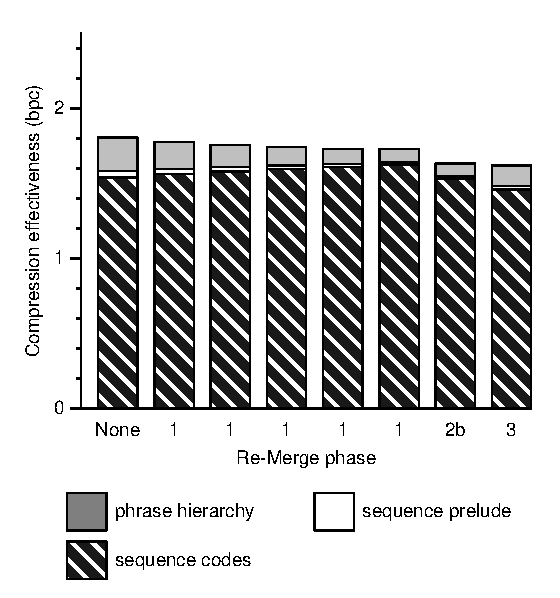
\includegraphics{./wsj-char-remerge-e.eps}
}{Compression ratios of character-based \repair and method E
of \remerge for \wsjb.  Each vertical bar represents the
initial compression with \repair, or a single application of
\remerge.  Initially, there are 26 blocks, which requires phase
1 five passes to combine into a single block.  Then,
phase 2b is applied, followed by phase 3.}{Compression ratios
for method E of \remerge (\wsjb)}
{fig:remerge-cb-bpc}

The compression, decompression, and block merging times for
character-based \repair with \wsjb are shown in 
\tabref{tab:remerge-cb-time}.  The time for phase 1 includes
all 5 iterations necessary to transform the 26 blocks into
a single block.  Of interest is the fact that
phase 2b takes 10 times longer than phase 2a.  However, when
phase 3 follows either (methods D and E), the time required
is similar, regardless of which version of phase 2 has been 
chosen.  In comparison to \repair and \remerge, the time
taken for sequence coding with \shuff is small.  As for
decoding, note that regardless of which type of encoding has
been chosen, the decoding requirements is small and always
between 70 and 80 seconds.  While phase 2b requires an average
of 3,276.5 seconds, a simpler approach that 
eliminated secondary prefix symbols and
extended symbols required an average of 5,994.5 seconds.  
This less principled approach retained an index to the primitives
and primary prefix symbols, though.

\tab{lrrrrrr}{
& \multicolumn{1}{c}{\multirow{2}*{None}} & \multicolumn{5}{c}{\remerge Method} \\ \cline{3-7}
                          & & \multicolumn{1}{c}{A} & \multicolumn{1}{c}{B} & \multicolumn{1}{c}{C} & \multicolumn{1}{c}{D} & \multicolumn{1}{c}{E} \\}
{
Encoding time      &         &         &         &         &         &         \\
{\D\D}\repair      & 2,323.3 & 2,323.3 & 2,323.3 & 2,323.3 & 2,323.3 & 2,323.3 \\
{\D\D}\remerge 1   &         &   453.0 &   453.0 &   453.0 &   453.0 &   453.0 \\
{\D\D}\remerge 2a  &         &         &   394.4 &         &   394.4 &         \\
{\D\D}\remerge 2b  &         &         &         & 3,276.5 &         & 3,276.5 \\
{\D\D}\remerge 3   &         &         &         &         &   222.2 &   202.5 \\
{\D\D}\shuff       &    39.2 &    32.1 &    31.0 &    30.6 &    34.3 &    32.7 \\
{\D\D}Total       & 2,362.5 & 2,808.4 & 3,201.7 & 6,083.4 & 3,427.2 & 6,288.0 \\
\\
Decoding time      &         &         &         &         &         &         \\
{\D\D}\shuff       &     9.3 &     8.1 &     8.3 &     8.9 &     9.3 &     9.2 \\
{\D\D}\despair     &    62.9 &    61.9 &    63.3 &    65.8 &    68.2 &    68.9 \\
{\D\D}Total        &    72.2 &    70.0 &    71.6 &    74.7 &    77.5 &    78.1 \\
}{Compression times for \remerge with character-based \repair on
\wsjb.
In the first column, ``None'' represents no block merging 
performed, using the output from \repair directly.  Times
are in CPU seconds on a \vipe, and averaged over three trials.}
{Compression times for \remerge with character-based \repair (\wsjb)}
{tab:remerge-cb-time}

The results from applying punctuation-aligned \repair to \news
are similar to those of character-based \repair to \wsjb.
The first step in punctuation-aligned \repair is the 
pre-processing stage with \prepair.  When a \remerge
configuration has been chosen, the only difference between it and any other
combination is the execution times and compression ratios of the
word sequence.  So, values related to the 
lexicons and the modifiers are constant.
These fixed values
are shown in \tabref{tab:remerge-pa-otherstats} and re-appear
in future tables in this chapter under the heading of ``Other''.

\tab{lccc}
{
                             & Compression & Encoding & Decoding \\
                             & (bpc)       & time (s)    & time (s) \\
}
{
\prepair                     & N/A      &    724.9 &    142.5 \\
Streams:                     &          &          &          \\
{\D\D}Word lexicon           & \E0.005    &  \D\D1.2 &  \D\D0.7 \\
{\D\D}Non-word lexicon       & {\tl}0.001 & \hphantom{,}{\tl}0.1 & \hphantom{,}{\tl}0.1 \\
{\D\D}Case-folding modifiers & \E0.240    &   \D16.2 &  \D\D7.1 \\
{\D\D}Stemming modifiers     & \E0.377    &   \D18.3 &  \D\D7.5 \\
{\D\D}Non-word modifiers     & \E0.342    &   \D16.6 &  \D\D7.3 \\
Total                        & \E0.964    &    777.2 &    165.1 \\
}{Compression ratios and execution times for the streams of 
\prepair, not including the word sequence stream, when applied
to \news.  The lexicons
have been front-coded and then compressed using \bzip.  The two
streams of modifiers and the non-word sequence have been 
compressed with \shuff, using a block size of 20,971,520 
symbols.  Execution times have been averaged over three trials.}
{Applying \prepair for \remerge (\news)}
{tab:remerge-pa-otherstats}

Some phrase hierarchy and sequence statistics pertaining to
punctuation-aligned \repair for \news are shown in 
\tabref{tab:remerge-pa-stats}.  \repair creates
nine blocks from the 168,721,097 symbols of the 
word sequence.  As with character-based \repair, between
the column ``None'' and method A, the phrase hierarchy's
size decreases.  Methods B and C both reduce the length
of the sequence, with method C being more effective.
Likewise, method E is an improvement to method D in
both the final sequence length and the number of phrases
required to achieve that length.  With \news, there are
no changes to the maximum generation in a block and
the length of the longest symbol.  The average length of
a segment during phase 2b was 5.5 primitives,
much less than for character-based \repair.

\tab{lrrrrrr}{
& \multicolumn{1}{c}{\multirow{2}*{None}} & \multicolumn{5}{c}{\remerge Method} \\ \cline{3-7}
                          & & \multicolumn{1}{c}{A} & \multicolumn{1}{c}{B} & \multicolumn{1}{c}{C} & \multicolumn{1}{c}{D} & \multicolumn{1}{c}{E} \\}
{
%%  Experiment:
$|\Sigma|$       &    848,016 &    336,739 &    336,739 &    336,739 &    336,739 &    336,739 \\
$|\rho|$         &  9,916,387 &  6,554,510 &  6,554,510 &  6,554,510 &  8,275,000 &  7,940,620 \\
$|\Seq'|$        & 67,097,856 & 67,097,848 & 63,709,684 & 61,734,292 & 59,932,869 & 58,685,281 \\
gen              &         25 &         25 &         25 &         25 &         25 &         25 \\ %% max in block
$|\alpha_L|$     &      1,348 &      1,348 &      1,348 &      1,348 &      1,348 &      1,348 \\ %% max in block
$b$              &          9 &          1 &          1 &          1 &          1 &          1 \\
}{Statistics for \remerge with punctuation-aligned \repair.  
The column marked ``None'' 
represents no block merging performed.  Primitives,
phrases, and the final sequence are abbreviated as
$\Sigma$, $\rho$, and $\Seq'$.  The
row marked ``gen'' is the maximum symbol generation in any
block, while $|\alpha_L|$ is the length of the longest
symbol, expressed in primitives.  The last row, $b$, is
the number of blocks.}
{Statistics for \remerge with punctuation-aligned \repair (\news)}
{tab:remerge-pa-stats}

The compression ratios of \tabref{tab:remerge-pa-bpc} reflect
the levels for character-based \repair, with one
notable exception.  While phase 3 has reduced the length of the
sequence, the compression ratios of methods D and E are worse
than those of methods B and C.  To be precise, the compression
ratios of the sequence for methods D and E have improved, but
not enough to compensate for the increase in size of the phrase
hierarchy.

\tab{lcccccc}{
& \multirow{2}*{None} & \multicolumn{5}{c}{\remerge Method} \\ \cline{3-7}
                    &       & A     & B     & C     & D     & E     \\}
{
Phrase hierarchy    & 0.163 & 0.116 & 0.116 & 0.116 & 0.143 & 0.138 \\
Sequence (\shuff)   & 1.145 & 1.181 & 1.159 & 1.153 & 1.137 & 1.131 \\
Other               & 0.964 & 0.964 & 0.964 & 0.964 & 0.964 & 0.964 \\
Total               & 2.272 & 2.261 & 2.239 & 2.233 & 2.244 & 2.233 \\
}{Compression ratios for \remerge with punctuation-aligned \repair.
In the second column, ``None'' represents no block merging 
performed, using the output from \repair directly.  In the sixth
row, ``Other'' represents the compression ratio of the other
streams, as shown in \tabref{tab:remerge-pa-otherstats}.}
{Compression levels for \remerge with punctuation-aligned \repair (\news)}
{tab:remerge-pa-bpc}

The execution times for punctuation-aligned \repair and \remerge are
presented in \tabref{tab:remerge-pa-time}.  For the total times, the
costs of encoding and decoding the modifiers 
have been taken into account in the rows marked ``Other''.  
The execution time difference
between methods are similar to the differences between methods for
character-based \repair.  And, as before, the decoding
times are fairly consistent, whether \repair alone has been applied, or
followed by a \remerge method.  

\tab{lrrrrrr}{
& \multicolumn{1}{c}{\multirow{2}*{None}} & \multicolumn{5}{c}{\remerge Method} \\ \cline{3-7}
                          & & \multicolumn{1}{c}{A} & \multicolumn{1}{c}{B} & \multicolumn{1}{c}{C} & \multicolumn{1}{c}{D} & \multicolumn{1}{c}{E} \\}
{
Encoding time      &         &         &         &         &         &         \\
{\D\D}Other        &   777.2 &   777.2 &   777.2 &   777.2 &   777.2 &   777.2 \\
{\D\D}\repair      & 1,634.3 & 1,634.3 & 1,634.3 & 1,634.3 & 1,634.3 & 1,634.3 \\
{\D\D}\remerge 1   &         &   636.7 &   636.7 &   636.7 &   636.7 &   636.7 \\
{\D\D}\remerge 2a  &         &         & 1,142.2 &         & 1,142.2 &         \\
{\D\D}\remerge 2b  &         &         &         & 2,645.4 &         & 2,645.4 \\
{\D\D}\remerge 3   &         &         &         &         &   312.1 &   288.8 \\
{\D\D}\shuff       &    55.0 &    51.4 &    50.5 &    50.0 &    53.4 &    52.3 \\
{\D\D}Total        & 2,466.5 & 3,099.6 & 4,240.9 & 5,743.6 & 4,555.9 & 6,034.7 \\
\\
Decoding time      &         &         &         &         &         &         \\
{\D\D}\shuff       &    13.3 &    12.3 &    12.4 &    12.9 &    13.7 &    13.5 \\
{\D\D}\despair     &    52.8 &    53.3 &    54.4 &    55.5 &    57.7 &    58.3 \\
{\D\D}Other        &   165.1 &   165.1 &   165.1 &   165.1 &   165.1 &   165.1 \\
{\D\D}Total        &   231.2 &   230.7 &   231.9 &   233.5 &   236.5 &   236.9 \\
}{Compression times for \remerge with punctuation-aligned \repair for
the file \news.
In the first column, ``None'' represents no block merging 
performed, using the output from \repair directly.  The rows
labelled ``Other'' represent the total compression times
of the other streams, as shown in \tabref{tab:remerge-pa-otherstats}.
Times are in CPU seconds on a \vipe.}
{Compression times for \remerge with punctuation-aligned \repair (\news)}
{tab:remerge-pa-time}

%%  Linking time for punctuation-aligned Re-Pair (Expt 582):
%%    1092.47 - 1053.68 = 38.79
%%    1093.36 - 1054.69 = 38.67
%%    1092.53 - 1053.88 = 38.65
%%  average:  38.7
%%  Linking time for character-based Re-Pair (Expt 576):
%%    83.65 - 74.39 = 9.26
%%    83.43 - 74.28 = 9.15
%%    83.51 - 74.23 = 9.28
%%  average:  9.2
The elementary approach to phase 2b
was also applied, and was actually found to be marginally faster.  Without 
secondary prefix symbols and extended symbols, 2,569.7 seconds 
was taken by \remerge, as opposed to 2,640.9 seconds.  The time to 
construct these symbol links for phase 2b was 38.7 seconds, 
on average.
There was no gain in time by adding these links partly due to the generally
shorter symbols than character-based \repair.  The longest symbol for
punctuation-aligned \repair had 1,348 word tokens, while the longest
symbol for character-based \repair consisted of 4,970 
characters.  In comparison,
the extra symbol linking time for character-based 
\repair was 9.2 seconds, which was easily justifiable
due to the improvements in speed.  While the
phrase hierarchy produced by punctuation-aligned \repair was larger,
since the primitives represent words, there was less similarity between
consecutive symbols in the phrase hierarchy sorted by expanded strings.
So, if memory constraints exists,
then choosing the simpler version of phase 2b would save 
$6 (|\Sigma| + |\rho|)$ words of memory for punctuation-aligned
\repair

\newsection{Appending to a Compressed Document}{sec:remerge-append}

The success of \remerge as a post-processor for \repair is due to
its memory usage.  While \repair requires enough space to hold the
entire message, each phase of \remerge occupies memory which is
proportional to the size of the phrase hierarchy.
In the experiments described above, \wsjb and \news
could be processed by \remerge on a test machine with \gib{1} 
of memory.  

Problems with \remerge arise if the phrase hierarchy of the
reduced message is larger than the amount of available memory.  
This section proposes a solution which involves the creation
of a phrase hierarchy from a subset of the message to act as training
data.  The size of the subset must be small enough so
that when it is post-processed with \remerge, the phrase hierarchy
can be kept within memory.  This phrase hierarchy
is then used to compress the remainder of the message through a technique
similar to phase 2b.  Hence, the time and space requirements for
appending text is same as for phase 2b.

Appending text to a compressed document
presents two problems.  First, the phrases created with the 
training data may not be representative of the rest of the
message.  As more text is processed with the static phrase hierarchy,
compression is expected to degrade.  Second, \remerge requires the
set of primitives to be known ahead of time.  Regardless of how much of
a message has been seen, the appearance
of a novel primitive can
always occur.  The structure of the phrase hierarchy and the method
with which it is encoded prevents symbols to be inserted in the middle.
Whenever a new symbol is added to the phrase hierarchy, the structure
must be re-built and the symbols in the sequence renumbered, as with
phase 3 of \remerge.  

The experiments described below respond to the first problem by demonstrating how
the size of the training data affects overall compression 
effectiveness.  Appending text with \remerge was implemented specifically
for character-based \repair.  As a result, the set of primitives is 
limited to the 256 characters of the \eascii
character set.  After the experiments, a proposed solution for 
word-based and punctuation-aligned \repair is discussed.

Appending text with \remerge is similar to the semi-static version of
\ray called \xray \citep{cw02:tis}.  The \xray algorithm creates a
dictionary using a portion of the message as training data.  Then,
this training data is applied on-line to the remainder of the
message.  After the training phase, Huffman codes are assigned to
the dictionary entries, so that phrase selection afterwards is based
on the lengths of the corresponding codewords.  A window of text
is examined at a time, and phrases are chosen based on the assignment
of a penalty for bypassing a replacement.  In contrast to \xray, 
\remerge continues to separate the phrase selection heuristic from
the entropy coder for the reduced word sequence, so that phrases are
selected based on how much the sequence length can be reduced.
As with phase 2b, each primitive from the second part of the message
is placed in a node in a DAG, and the shortest path through
is determined by following edges representing phrase hierarchy symbols.

In order to measure the performance of appending text,
character-based \repair was used to compress \wsjb.  Various sizes of
training data were taken from the front of \wsjb and partitioned into
blocks of \mib{20} each.  These blocks were merged using method E of
\remerge.  That is, all of the blocks were combined through multiple 
iterations of phase 1, followed by phase 2b, and then phase 3.  
The remainder of \wsjb is then appended to the end of the reduced 
training data.  An alternative experimental framework would obtain
the training data from random sections within \wsjb.  While
the current implementation of \remerge would support this approach,
it was not used because the articles within \wsjb are ordered 
chronologically.  Appending text gives the illusion that new documents
are being added to the collection over time.

\tabref{tab:remerge-append-stats} provides statistics from these
experiments after all of \wsjb has been processed.
For each training size ranging from \mib{20} to \mib{400},
the number of primitives, the number of phrases, the length of
the final sequence, the length of the longest phrase
in primitives, and the maximum generation are presented.
The last row of the table is obtained from earlier experiments
with character-based \repair and \wsjb 
(see the column marked ``method E'' in 
\tabref{tab:remerge-cb-stats}).  Those experiments are equivalent
to making all of \wsjb the training data.

\tab{cccccc}{
Training size & \multirow{2}*{$|\Sigma|$} & \multirow{2}*{$|\rho|$} & \multirow{2}*{$|\Seq'|$} & \multirow{2}*{$|\alpha_L|$} & \multirow{2}*{gen} \\
(\mibonly) & & & & & \\
}
{
\D20 & 256 & \C322,432 & 71,240,604 & 1,257 & 21 \\
\D40 & 256 & \C552,784 & 65,724,383 & 1,257 & 22 \\
\D80 & 256 & \C948,903 & 60,802,497 & 2,084 & 21 \\
120  & 256 & 1,302,459 & 58,221,318 & 4,970 & 21 \\
160  & 256 & 1,647,723 & 55,121,237 & 4,970 & 23 \\
240  & 256 & 2,278,342 & 52,039,645 & 4,970 & 24 \\
320  & 256 & 2,905,923 & 44,730,578 & 4,970 & 27 \\
400  & 256 & 3,467,728 & 40,738,832 & 4,970 & 28 \\
508  & \D94& 4,164,166 & 38,955,830 & 4,970 & 28 \\
}{Statistics for appending text with character-based \repair
on \wsjb.  The first column indicates the size of
the training data.  Then,
$\Sigma$, $\rho$, and $\Seq'$ represent the
primitives, phrases, and final sequence, respectively.  The
column marked $|\alpha_L|$ is the length of the longest phrase
in primitives, and ``gen'' is the maximum symbol generation.}
{Statistics for appending text with character-based \repair (\wsjb)}
{tab:remerge-append-stats}

As \tabref{tab:remerge-append-stats} shows, as more 
training data is used, the number of phrases, the maximum phrase length,
and the maximum generation increase.  Also, since the phrase hierarchy
contains more symbols, the length of the sequence becomes shorter.
Note that the number of primitives is always fixed at 256.  In the
last row, when all of the message is seen, the space allocated to
generation 0 is equal to the number of distinct primitives that appear
in the message.

\figref{fig:remerge-append} presents the compression levels 
achieved as a function of the size of the training data.
The compressed sizes are calculated from the merged training data,
and again once the rest of \wsjb has been appended.  In both
cases, the reduced sequence was encoded with \shuff as a single
block.  As expected, overall 
compression effectiveness improves as the training set 
increases in size.  The best compression
ratio on the graph is achieved when the initial training size is
equal to the size of \wsjb.  However, with just 16\% of \wsjb
used as training data,
the compression effectiveness achieved is only 18\% worse
than applying \repair and \remerge on the entire file.

\fig{\includegraphics*{./wsj-char-append.eps}}
{Compression effectiveness of \remerge when appending text 
to various sizes of training data using character-based \repair
and the \wsjb test file.  The initial block size for \repair is
\mib{20}.  The solid line represents the compression effectiveness
of the entire file, while the dashed line indicates the size of
the compressed training data.}
{Compression effectiveness of \remerge for appending text (\wsjb)}
{fig:remerge-append}

The time required to compress \wsjb is presented in 
\tabref{tab:remerge-append-encode}.  As the size of the training
data increases, the time required to apply both \repair and
method E of \remerge also increases.  While \remerge is not necessary
for the training size of \mib{20}, it was applied in order to remove
any duplicates in the phrase hierarchy.  The time required to append
the remaining text does not increase in a similar manner, though.  
After a certain training size, the cost of appending is 
offset by the amount of text left to add.
The time required to append text peaks
when the training size is \mib{80}.  The time taken to encode the
reduced sequence with \shuff is similar throughout the
experiment.  Regardless of the costs of appending and sequence encoding,
the dominant times belong to \repair and method E of \remerge.  
Because of this, the total time increases with the training size.

\tab{cccccc}
{
Training size & \multirow{2}*{\repair} & \remerge & Append & \multirow{2}*{\shuff} & \multirow{2}*{Total} \\
(\mibonly) &         & (method E) & text &       & \\
}
{
\D20&     \C\D88.7       &  \C114.6  & 2,662.3 & 31.6   & 2,897.2 \\
\D40&      \C180.0       &  \C186.3  & 2,937.7 & 31.3   & 3,335.3 \\
\D80&      \C363.0       &  \C428.1  & 3,165.7 & 31.5   & 3,988.3 \\
120 &      \C546.4       &  \C708.5  & 3,126.0 & 31.6   & 4,412.5 \\
160 &      \C732.3       &  \C981.4  & 2,986.1 & 31.8   & 4,731.6 \\
240 &       1,102.5      &  1,610.9   & 2,457.6 & 32.0   & 5,203.0 \\
320 &       1,467.2      &  2,246.2   & 1,891.2 & 31.6   & 5,636.2 \\
400 &       1,834.2      &  2,954.3   & 1,200.5 & 31.6   & 6,020.6 \\
508 &       2,323.3      &  3,932.0   & ---     & 32.7   & 6,288.0 \\
}{Encoding times for character-based \repair and appending with \remerge
for various sizes of training data.  Times are in CPU seconds and 
averaged over three trials on a \vipe.}{Encoding times for 
appending text with character-based \repair (\wsjb)}
{tab:remerge-append-encode}

The decompression times for appending text are given in
\tabref{tab:remerge-append-decode}.  The decoding time of \shuff 
and the phrase expansion time of \despair both increase as the training
data becomes larger.  This increase is due to the larger phrase 
hierarchy, despite the sequence becoming shorter.

\tab{cccc}
{
Training size & \multirow{2}*{\shuff} & \multirow{2}*{\despair} & \multirow{2}*{Total} \\
(\mibonly)        &          &        & \\
}
{
\D20 & 7.0   & 56.0      & 63.0 \\
\D40 & 7.3   & 57.4      & 64.7 \\
\D80 & 7.7   & 59.7      & 67.4 \\
120  & 7.8   & 61.3      & 69.1 \\
160  & 8.1   & 62.2      & 70.3 \\
240  & 8.3   & 62.9      & 71.2 \\
320  & 8.6   & 64.4      & 73.0 \\
400  & 8.7   & 65.8      & 74.5 \\
508  & 9.2   & 68.2      & 78.1 \\
}{Times for decoding a compressed message made with character-based
\repair with various sizes of training data.
Times are in CPU seconds and averaged
over three trials on a \vipe.}
{Decoding times for appending text with character-based \repair (\wsjb)}
{tab:remerge-append-decode}

The addition of text to a compressed message serves two purposes.
The first, as mentioned already, is to enable documents which
yield a large phrase hierarchy to be processed.  The second purpose 
is to support dynamic collections, where new documents 
are added to the repository
throughout its lifetime.  The coding mechanism provided by 
\shuff does not allow periodic additions to the compressed 
sequence, and the solution adopted by the experiments is to 
re-encode the sequence after any changes.  An alternative is to
apply \shuff in blocks, and make each extension a block.
Otherwise, support of
both aims for character-based \repair is complete.

The problem becomes more complicated for word-based and
punctuation-aligned \repair, since no restriction is
placed on the number of unique words.  When a novel word appears,
it must be added to the word lexicon.  However, since the positions in
the lexically sorted word lexicon are used to create the word sequence
for \repair, both streams must be recompressed.  A similar problem occurs
when a novel non-word symbol appears in the message.

\citet{mzs97:tkde}
discusses several solutions for compressing dynamic document databases,
two of which can be adapted for \repair.  The first idea adds an escape
symbol which signals to the decoder that the following is a novel word,
specified using a secondary model, such as characters.  While
this idea permits dynamic document compression, the loss of the word 
boundaries enforced by \prepair make it unsuitable for browsing.
The second method proposed by \citeauthor{mzs97:tkde}\ would also
introduce an escape primitive to the phrase hierarchy, except that 
the escape symbol forces 
the decoder to consult an auxiliary word lexicon.  This secondary word
lexicon is unsorted, and no limit is placed on its size.  However, because
of the compact nature of \repair's phrase hierarchy, these words cannot be
used to form phrases.  One way of circumventing this problem is to extend
the escape mechanism to phrases.
Whenever an escape is encountered while expanding the reduced
word sequence, the auxiliary phrase hierarchy is consulted instead.

The ideal method of compression for the unstructured auxiliary phrase
hierarchy is undetermined at this time and appending of text 
with word-based or punctuation-aligned \repair requires
further investigation.

\newsection{Summary}{sec:remerge-summary}

This chapter has described \remerge as a post-processing 
step to \repair.  When the source message is too large, it
must be compressed as independent blocks by \repair and then
merged with \remerge.
\remerge is feasible because each phase requires memory
proportional to the size of the phrase hierarchy.  This is in
contrast to \repair, whose memory usage is related to the
length of the message.  Even so, a message could be so large
that its corresponding phrase hierarchy exceeds the amount of
memory available.  This problem was considered 
for character-based \repair.
Adapting this solution for word-based and punctuation-aligned 
\repair is reserved for future work.

The block merging techniques of this chapter serve
three major goals.  The first goal is to enable
phrase browsing by combining multiple phrase hierarchies into 
a single one.  The second goal is to improve compression 
effectiveness through the removal of duplicates in the phrase
hierarchy and the identification of old and new symbol pairs
for replacement.  In satisfying the second goal, a third
objective emerges, since the quality of the symbols in the 
phrase hierarchy is improved as more symbol pairs are replaced.

The experiments in this chapter have shown that to achieve
these goals, no single best combination of \remerge phases
exists.  The three phases of
\remerge have been organised into five methods which 
illustrate the trade-offs between program execution time
and compression effectiveness.  All five methods satisfy
the first goal by outputting a unified phrase hierarchy.  
However, achieving the second and third targets requires
considerable additional computation time.  From the 
perspective of phrase browsing, a reduced
message that has been post-processed by any of the five
methods of \remerge can be browsed.  Which method should
be chosen depends on the amount of time available, and
on the compression effectiveness and phrase hierarchy
quality that is required.

The results from the experiments with punctuation-aligned
\repair and \news have been summarised in 
\figref{fig:remerge-throughput}.  The
graph plots the compression effectiveness of
\repair and the five methods of \remerge against their
throughput (number of bytes processed per second).

\fig{
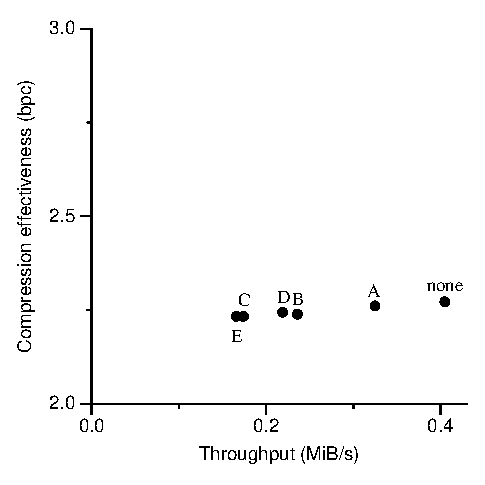
\includegraphics{./throughput.eps}
}{Graph of compression effectiveness versus throughput for
the previous section's experiments with 
punctuation-aligned \repair on the \news file for
the five methods of \remerge.  Times are for encoding, and
are measured on a \vipe.}
{Compression effectiveness versus throughput for \remerge (\news)}
{fig:remerge-throughput}

The emphasis in this thesis is on phrase browsing, and for the
remainder of this investigation method E for punctuation-aligned
\repair is the preferred approach.  While this method is expensive
with respect to compression speed, decompression time is unaffected
by this decision.

Chapters \ref{chap:repair}, \ref{chap:prepair}, and \ref{chap:remerge}
have not considered sequence and modifier coding.
The coding of these two types of streams is
addressed in \chapref{chap:review}, by first considering the 
problems inherent in the method chosen so far (Huffman coding
with \shuff) and then by proposing two alternative coding 
schemes.  

